\documentclass[twoside]{book}

% Packages required by doxygen
\usepackage{calc}
\usepackage{doxygen}
\usepackage{graphicx}
\usepackage[utf8]{inputenc}
\usepackage{makeidx}
\usepackage{multicol}
\usepackage{multirow}
\usepackage{textcomp}
\usepackage[table]{xcolor}

% Font selection
\usepackage[T1]{fontenc}
\usepackage{mathptmx}
\usepackage[scaled=.90]{helvet}
\usepackage{courier}
\usepackage{amssymb}
\usepackage{sectsty}
\renewcommand{\familydefault}{\sfdefault}
\allsectionsfont{%
  \fontseries{bc}\selectfont%
  \color{darkgray}%
}
\renewcommand{\DoxyLabelFont}{%
  \fontseries{bc}\selectfont%
  \color{darkgray}%
}

% Page & text layout
\usepackage{geometry}
\geometry{%
  a4paper,%
  top=2.5cm,%
  bottom=2.5cm,%
  left=2.5cm,%
  right=2.5cm%
}
\tolerance=750
\hfuzz=15pt
\hbadness=750
\setlength{\emergencystretch}{15pt}
\setlength{\parindent}{0cm}
\setlength{\parskip}{0.2cm}
\makeatletter
\renewcommand{\paragraph}{%
  \@startsection{paragraph}{4}{0ex}{-1.0ex}{1.0ex}{%
    \normalfont\normalsize\bfseries\SS@parafont%
  }%
}
\renewcommand{\subparagraph}{%
  \@startsection{subparagraph}{5}{0ex}{-1.0ex}{1.0ex}{%
    \normalfont\normalsize\bfseries\SS@subparafont%
  }%
}
\makeatother

% Headers & footers
\usepackage{fancyhdr}
\pagestyle{fancyplain}
\fancyhead[LE]{\fancyplain{}{\bfseries\thepage}}
\fancyhead[CE]{\fancyplain{}{}}
\fancyhead[RE]{\fancyplain{}{\bfseries\leftmark}}
\fancyhead[LO]{\fancyplain{}{\bfseries\rightmark}}
\fancyhead[CO]{\fancyplain{}{}}
\fancyhead[RO]{\fancyplain{}{\bfseries\thepage}}
\fancyfoot[LE]{\fancyplain{}{}}
\fancyfoot[CE]{\fancyplain{}{}}
\fancyfoot[RE]{\fancyplain{}{\bfseries\scriptsize Generated on Wed Jun 5 2013 23:54:58 for cards-with-friends by Doxygen }}
\fancyfoot[LO]{\fancyplain{}{\bfseries\scriptsize Generated on Wed Jun 5 2013 23:54:58 for cards-with-friends by Doxygen }}
\fancyfoot[CO]{\fancyplain{}{}}
\fancyfoot[RO]{\fancyplain{}{}}
\renewcommand{\footrulewidth}{0.4pt}
\renewcommand{\chaptermark}[1]{%
  \markboth{#1}{}%
}
\renewcommand{\sectionmark}[1]{%
  \markright{\thesection\ #1}%
}

% Indices & bibliography
\usepackage{natbib}
\usepackage[titles]{tocloft}
\setcounter{tocdepth}{3}
\setcounter{secnumdepth}{5}
\makeindex

% Hyperlinks (required, but should be loaded last)
\usepackage{ifpdf}
\ifpdf
  \usepackage[pdftex,pagebackref=true]{hyperref}
\else
  \usepackage[ps2pdf,pagebackref=true]{hyperref}
\fi
\hypersetup{%
  colorlinks=true,%
  linkcolor=blue,%
  citecolor=blue,%
  unicode%
}

% Custom commands
\newcommand{\clearemptydoublepage}{%
  \newpage{\pagestyle{empty}\cleardoublepage}%
}


%===== C O N T E N T S =====

\begin{document}

% Titlepage & ToC
\hypersetup{pageanchor=false}
\pagenumbering{roman}
\begin{titlepage}
\vspace*{7cm}
\begin{center}%
{\Large cards-\/with-\/friends }\\
\vspace*{1cm}
{\large Generated by Doxygen 1.8.4}\\
\vspace*{0.5cm}
{\small Wed Jun 5 2013 23:54:58}\\
\end{center}
\end{titlepage}
\clearemptydoublepage
\tableofcontents
\clearemptydoublepage
\pagenumbering{arabic}
\hypersetup{pageanchor=true}

%--- Begin generated contents ---
\chapter{cards-\/with-\/friends}
\label{md_README}
\hypertarget{md_README}{}
Cards with Friends 
\chapter{Hierarchical Index}
\section{Class Hierarchy}
This inheritance list is sorted roughly, but not completely, alphabetically\-:\begin{DoxyCompactList}
\item dict\begin{DoxyCompactList}
\item \contentsline{section}{cards-\/with-\/friends.pylib.\-utils.\-Attribute\-Dict}{\pageref{classcards-with-friends_1_1pylib_1_1utils_1_1_attribute_dict}}{}
\end{DoxyCompactList}
\item Iterator\begin{DoxyCompactList}
\item \contentsline{section}{cards-\/with-\/friends.deck.\-Deck}{\pageref{classcards-with-friends_1_1deck_1_1_deck}}{}
\end{DoxyCompactList}
\item object\begin{DoxyCompactList}
\item \contentsline{section}{cards-\/with-\/friends.card.\-Card}{\pageref{classcards-with-friends_1_1card_1_1_card}}{}
\item \contentsline{section}{cards-\/with-\/friends.main.\-Room}{\pageref{classcards-with-friends_1_1main_1_1_room}}{}
\item \contentsline{section}{cards-\/with-\/friends.pylib.\-mixins.\-Message\-Mixin}{\pageref{classcards-with-friends_1_1pylib_1_1mixins_1_1_message_mixin}}{}
\end{DoxyCompactList}
\item Base\-Namespace\begin{DoxyCompactList}
\item \contentsline{section}{cards-\/with-\/friends.main.\-Card\-Namespace}{\pageref{classcards-with-friends_1_1main_1_1_card_namespace}}{}
\end{DoxyCompactList}
\item Broadcast\-Mixin\begin{DoxyCompactList}
\item \contentsline{section}{cards-\/with-\/friends.main.\-Card\-Namespace}{\pageref{classcards-with-friends_1_1main_1_1_card_namespace}}{}
\end{DoxyCompactList}
\item Game\begin{DoxyCompactList}
\item \contentsline{section}{cards-\/with-\/friends.trick\-\_\-taking\-\_\-game.\-Trick\-Taking\-Game}{\pageref{classcards-with-friends_1_1trick__taking__game_1_1_trick_taking_game}}{}
\end{DoxyCompactList}
\item Message\-Mixin\begin{DoxyCompactList}
\item \contentsline{section}{cards-\/with-\/friends.game.\-Game}{\pageref{classcards-with-friends_1_1game_1_1_game}}{}
\item \contentsline{section}{cards-\/with-\/friends.main.\-Game\-Manager}{\pageref{classcards-with-friends_1_1main_1_1_game_manager}}{}
\item \contentsline{section}{cards-\/with-\/friends.player.\-\_\-\-Hand}{\pageref{classcards-with-friends_1_1player_1_1___hand}}{}
\item \contentsline{section}{cards-\/with-\/friends.player.\-Player}{\pageref{classcards-with-friends_1_1player_1_1_player}}{}
\end{DoxyCompactList}
\item Rooms\-Mixin\begin{DoxyCompactList}
\item \contentsline{section}{cards-\/with-\/friends.main.\-Card\-Namespace}{\pageref{classcards-with-friends_1_1main_1_1_card_namespace}}{}
\end{DoxyCompactList}
\item Trick\-Taking\-Game\begin{DoxyCompactList}
\item \contentsline{section}{cards-\/with-\/friends.games.\-hearts.\-Hearts}{\pageref{classcards-with-friends_1_1games_1_1hearts_1_1_hearts}}{}
\item \contentsline{section}{cards-\/with-\/friends.games.\-highest\-\_\-card.\-Highest\-Card}{\pageref{classcards-with-friends_1_1games_1_1highest__card_1_1_highest_card}}{}
\item \contentsline{section}{cards-\/with-\/friends.games.\-spades.\-Spades}{\pageref{classcards-with-friends_1_1games_1_1spades_1_1_spades}}{}
\end{DoxyCompactList}
\end{DoxyCompactList}

\chapter{Class Index}
\section{Class List}
Here are the classes, structs, unions and interfaces with brief descriptions\-:\begin{DoxyCompactList}
\item\contentsline{section}{\hyperlink{classcards-with-friends_1_1player_1_1___hand}{cards-\/with-\/friends.\-player.\-\_\-\-Hand} }{\pageref{classcards-with-friends_1_1player_1_1___hand}}{}
\item\contentsline{section}{\hyperlink{classcards-with-friends_1_1pylib_1_1utils_1_1_attribute_dict}{cards-\/with-\/friends.\-pylib.\-utils.\-Attribute\-Dict} }{\pageref{classcards-with-friends_1_1pylib_1_1utils_1_1_attribute_dict}}{}
\item\contentsline{section}{\hyperlink{classcards-with-friends_1_1card_1_1_card}{cards-\/with-\/friends.\-card.\-Card} }{\pageref{classcards-with-friends_1_1card_1_1_card}}{}
\item\contentsline{section}{\hyperlink{classcards-with-friends_1_1main_1_1_card_namespace}{cards-\/with-\/friends.\-main.\-Card\-Namespace} }{\pageref{classcards-with-friends_1_1main_1_1_card_namespace}}{}
\item\contentsline{section}{\hyperlink{classcards-with-friends_1_1deck_1_1_deck}{cards-\/with-\/friends.\-deck.\-Deck} }{\pageref{classcards-with-friends_1_1deck_1_1_deck}}{}
\item\contentsline{section}{\hyperlink{classcards-with-friends_1_1game_1_1_game}{cards-\/with-\/friends.\-game.\-Game} }{\pageref{classcards-with-friends_1_1game_1_1_game}}{}
\item\contentsline{section}{\hyperlink{classcards-with-friends_1_1main_1_1_game_manager}{cards-\/with-\/friends.\-main.\-Game\-Manager} \\*C\-L\-A\-S\-S\-E\-S }{\pageref{classcards-with-friends_1_1main_1_1_game_manager}}{}
\item\contentsline{section}{\hyperlink{classcards-with-friends_1_1games_1_1hearts_1_1_hearts}{cards-\/with-\/friends.\-games.\-hearts.\-Hearts} }{\pageref{classcards-with-friends_1_1games_1_1hearts_1_1_hearts}}{}
\item\contentsline{section}{\hyperlink{classcards-with-friends_1_1games_1_1highest__card_1_1_highest_card}{cards-\/with-\/friends.\-games.\-highest\-\_\-card.\-Highest\-Card} }{\pageref{classcards-with-friends_1_1games_1_1highest__card_1_1_highest_card}}{}
\item\contentsline{section}{\hyperlink{classcards-with-friends_1_1pylib_1_1mixins_1_1_message_mixin}{cards-\/with-\/friends.\-pylib.\-mixins.\-Message\-Mixin} }{\pageref{classcards-with-friends_1_1pylib_1_1mixins_1_1_message_mixin}}{}
\item\contentsline{section}{\hyperlink{classcards-with-friends_1_1player_1_1_player}{cards-\/with-\/friends.\-player.\-Player} }{\pageref{classcards-with-friends_1_1player_1_1_player}}{}
\item\contentsline{section}{\hyperlink{classcards-with-friends_1_1main_1_1_room}{cards-\/with-\/friends.\-main.\-Room} }{\pageref{classcards-with-friends_1_1main_1_1_room}}{}
\item\contentsline{section}{\hyperlink{classcards-with-friends_1_1games_1_1spades_1_1_spades}{cards-\/with-\/friends.\-games.\-spades.\-Spades} }{\pageref{classcards-with-friends_1_1games_1_1spades_1_1_spades}}{}
\item\contentsline{section}{\hyperlink{classcards-with-friends_1_1trick__taking__game_1_1_trick_taking_game}{cards-\/with-\/friends.\-trick\-\_\-taking\-\_\-game.\-Trick\-Taking\-Game} }{\pageref{classcards-with-friends_1_1trick__taking__game_1_1_trick_taking_game}}{}
\end{DoxyCompactList}

\chapter{Class Documentation}
\hypertarget{classcards-with-friends_1_1player_1_1___hand}{\section{cards-\/with-\/friends.player.\-\_\-\-Hand Class Reference}
\label{classcards-with-friends_1_1player_1_1___hand}\index{cards-\/with-\/friends.\-player.\-\_\-\-Hand@{cards-\/with-\/friends.\-player.\-\_\-\-Hand}}
}
Inheritance diagram for cards-\/with-\/friends.player.\-\_\-\-Hand\-:\begin{figure}[H]
\begin{center}
\leavevmode
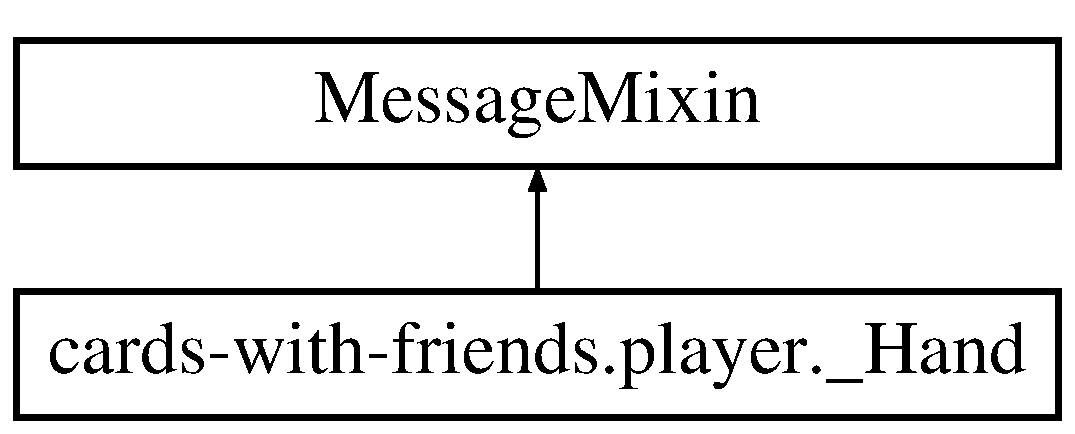
\includegraphics[height=2.000000cm]{classcards-with-friends_1_1player_1_1___hand}
\end{center}
\end{figure}
\subsection*{Public Member Functions}
\begin{DoxyCompactItemize}
\item 
\hypertarget{classcards-with-friends_1_1player_1_1___hand_a5fd754d851506c684339ff0aa39d04ba}{def {\bfseries \-\_\-\-\_\-init\-\_\-\-\_\-}}\label{classcards-with-friends_1_1player_1_1___hand_a5fd754d851506c684339ff0aa39d04ba}

\item 
\hypertarget{classcards-with-friends_1_1player_1_1___hand_a743c6f2318fb0758c5d8efc4f2432859}{def {\bfseries \-\_\-\-\_\-contains\-\_\-\-\_\-}}\label{classcards-with-friends_1_1player_1_1___hand_a743c6f2318fb0758c5d8efc4f2432859}

\item 
\hypertarget{classcards-with-friends_1_1player_1_1___hand_a892734bd2161656d006413916d9cd9d3}{def {\bfseries \-\_\-\-\_\-iter\-\_\-\-\_\-}}\label{classcards-with-friends_1_1player_1_1___hand_a892734bd2161656d006413916d9cd9d3}

\item 
\hypertarget{classcards-with-friends_1_1player_1_1___hand_acbf1685050647cf5701155c37f32d1d9}{def {\bfseries \-\_\-\-\_\-len\-\_\-\-\_\-}}\label{classcards-with-friends_1_1player_1_1___hand_acbf1685050647cf5701155c37f32d1d9}

\item 
\hypertarget{classcards-with-friends_1_1player_1_1___hand_a5a85b2b067c484cb58f55354526efd4b}{def {\bfseries \-\_\-\-\_\-nonzero\-\_\-\-\_\-}}\label{classcards-with-friends_1_1player_1_1___hand_a5a85b2b067c484cb58f55354526efd4b}

\item 
\hypertarget{classcards-with-friends_1_1player_1_1___hand_a5896a3a771c62190388d46644b0a7a41}{def {\bfseries \-\_\-\-\_\-repr\-\_\-\-\_\-}}\label{classcards-with-friends_1_1player_1_1___hand_a5896a3a771c62190388d46644b0a7a41}

\item 
def \hyperlink{classcards-with-friends_1_1player_1_1___hand_a1be4582215f118550b9a0699c5df3129}{Add}
\item 
def \hyperlink{classcards-with-friends_1_1player_1_1___hand_ad39478c86a8ca6fc2df6d0183fbc6a24}{Clear}
\item 
def \hyperlink{classcards-with-friends_1_1player_1_1___hand_a7c2eeab80d852bdf190addb5c3b2d3e5}{Remove}
\item 
\hypertarget{classcards-with-friends_1_1player_1_1___hand_aba6f65ae78d2e64f7d5a304fe59baede}{def {\bfseries player}}\label{classcards-with-friends_1_1player_1_1___hand_aba6f65ae78d2e64f7d5a304fe59baede}

\end{DoxyCompactItemize}


\subsection{Detailed Description}
\begin{DoxyVerb}A player's hand.\end{DoxyVerb}
 

\subsection{Member Function Documentation}
\hypertarget{classcards-with-friends_1_1player_1_1___hand_a1be4582215f118550b9a0699c5df3129}{\index{cards-\/with-\/friends\-::player\-::\-\_\-\-Hand@{cards-\/with-\/friends\-::player\-::\-\_\-\-Hand}!Add@{Add}}
\index{Add@{Add}!cards-with-friends::player::_Hand@{cards-\/with-\/friends\-::player\-::\-\_\-\-Hand}}
\subsubsection[{Add}]{\setlength{\rightskip}{0pt plus 5cm}def cards-\/with-\/friends.\-player.\-\_\-\-Hand.\-Add (
\begin{DoxyParamCaption}
\item[{}]{self, }
\item[{}]{cards}
\end{DoxyParamCaption}
)}}\label{classcards-with-friends_1_1player_1_1___hand_a1be4582215f118550b9a0699c5df3129}
\begin{DoxyVerb}Add one or more cards to the player's hand.\end{DoxyVerb}
 \hypertarget{classcards-with-friends_1_1player_1_1___hand_ad39478c86a8ca6fc2df6d0183fbc6a24}{\index{cards-\/with-\/friends\-::player\-::\-\_\-\-Hand@{cards-\/with-\/friends\-::player\-::\-\_\-\-Hand}!Clear@{Clear}}
\index{Clear@{Clear}!cards-with-friends::player::_Hand@{cards-\/with-\/friends\-::player\-::\-\_\-\-Hand}}
\subsubsection[{Clear}]{\setlength{\rightskip}{0pt plus 5cm}def cards-\/with-\/friends.\-player.\-\_\-\-Hand.\-Clear (
\begin{DoxyParamCaption}
\item[{}]{self}
\end{DoxyParamCaption}
)}}\label{classcards-with-friends_1_1player_1_1___hand_ad39478c86a8ca6fc2df6d0183fbc6a24}
\begin{DoxyVerb}Remove all cards from the player's hand.\end{DoxyVerb}
 \hypertarget{classcards-with-friends_1_1player_1_1___hand_a7c2eeab80d852bdf190addb5c3b2d3e5}{\index{cards-\/with-\/friends\-::player\-::\-\_\-\-Hand@{cards-\/with-\/friends\-::player\-::\-\_\-\-Hand}!Remove@{Remove}}
\index{Remove@{Remove}!cards-with-friends::player::_Hand@{cards-\/with-\/friends\-::player\-::\-\_\-\-Hand}}
\subsubsection[{Remove}]{\setlength{\rightskip}{0pt plus 5cm}def cards-\/with-\/friends.\-player.\-\_\-\-Hand.\-Remove (
\begin{DoxyParamCaption}
\item[{}]{self, }
\item[{}]{cards}
\end{DoxyParamCaption}
)}}\label{classcards-with-friends_1_1player_1_1___hand_a7c2eeab80d852bdf190addb5c3b2d3e5}
\begin{DoxyVerb}Remove one or more cards from the player's hand.\end{DoxyVerb}
 

The documentation for this class was generated from the following file\-:\begin{DoxyCompactItemize}
\item 
player.\-py\end{DoxyCompactItemize}

\hypertarget{classcards-with-friends_1_1pylib_1_1utils_1_1_attribute_dict}{\section{cards-\/with-\/friends.pylib.\-utils.\-Attribute\-Dict Class Reference}
\label{classcards-with-friends_1_1pylib_1_1utils_1_1_attribute_dict}\index{cards-\/with-\/friends.\-pylib.\-utils.\-Attribute\-Dict@{cards-\/with-\/friends.\-pylib.\-utils.\-Attribute\-Dict}}
}
Inheritance diagram for cards-\/with-\/friends.pylib.\-utils.\-Attribute\-Dict\-:\begin{figure}[H]
\begin{center}
\leavevmode
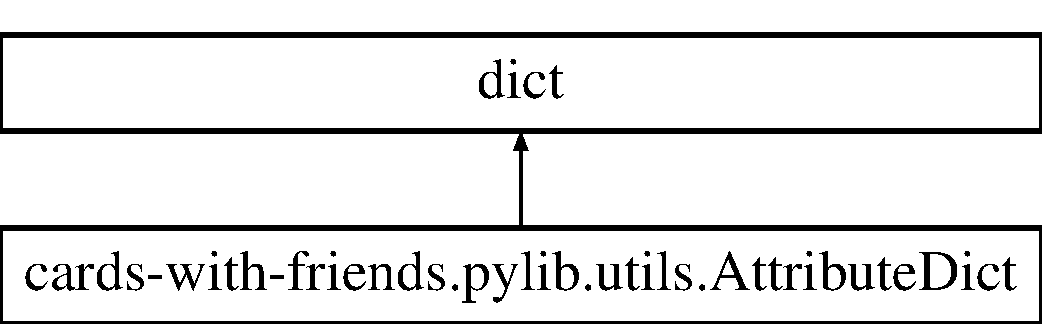
\includegraphics[height=2.000000cm]{classcards-with-friends_1_1pylib_1_1utils_1_1_attribute_dict}
\end{center}
\end{figure}
\subsection*{Public Member Functions}
\begin{DoxyCompactItemize}
\item 
\hypertarget{classcards-with-friends_1_1pylib_1_1utils_1_1_attribute_dict_a3e07d5952f9f7bc7469bcc30cecc9a96}{def {\bfseries \-\_\-\-\_\-init\-\_\-\-\_\-}}\label{classcards-with-friends_1_1pylib_1_1utils_1_1_attribute_dict_a3e07d5952f9f7bc7469bcc30cecc9a96}

\end{DoxyCompactItemize}


\subsection{Detailed Description}
\begin{DoxyVerb}Allow keys of a dictionary to be accessed like attributes.\end{DoxyVerb}
 

The documentation for this class was generated from the following file\-:\begin{DoxyCompactItemize}
\item 
pylib/utils.\-py\end{DoxyCompactItemize}

\hypertarget{classcards-with-friends_1_1card_1_1_card}{\section{cards-\/with-\/friends.card.\-Card Class Reference}
\label{classcards-with-friends_1_1card_1_1_card}\index{cards-\/with-\/friends.\-card.\-Card@{cards-\/with-\/friends.\-card.\-Card}}
}
Inheritance diagram for cards-\/with-\/friends.card.\-Card\-:\begin{figure}[H]
\begin{center}
\leavevmode
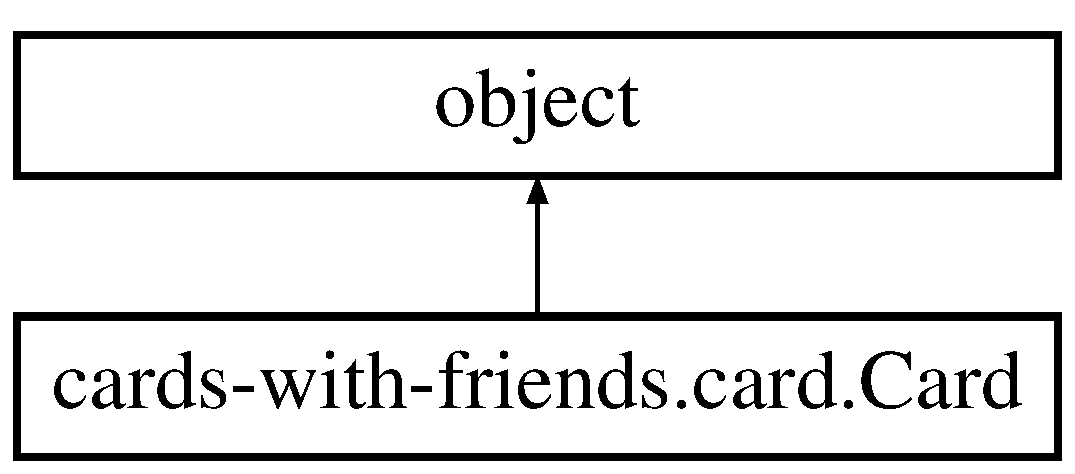
\includegraphics[height=2.000000cm]{classcards-with-friends_1_1card_1_1_card}
\end{center}
\end{figure}
\subsection*{Public Member Functions}
\begin{DoxyCompactItemize}
\item 
\hypertarget{classcards-with-friends_1_1card_1_1_card_a9a88beb1e241dc7392dd6f982fadc8c1}{def {\bfseries \-\_\-\-\_\-init\-\_\-\-\_\-}}\label{classcards-with-friends_1_1card_1_1_card_a9a88beb1e241dc7392dd6f982fadc8c1}

\item 
\hypertarget{classcards-with-friends_1_1card_1_1_card_ae903952193cd6f5bbd11efe200d17a65}{def {\bfseries \-\_\-\-\_\-eq\-\_\-\-\_\-}}\label{classcards-with-friends_1_1card_1_1_card_ae903952193cd6f5bbd11efe200d17a65}

\item 
\hypertarget{classcards-with-friends_1_1card_1_1_card_aa0346c601f6a98da90da1e9df60164aa}{def {\bfseries \-\_\-\-\_\-getattribute\-\_\-\-\_\-}}\label{classcards-with-friends_1_1card_1_1_card_aa0346c601f6a98da90da1e9df60164aa}

\item 
\hypertarget{classcards-with-friends_1_1card_1_1_card_a4804190fbe1caa433c0acf9f8c2c8945}{def {\bfseries \-\_\-\-\_\-ne\-\_\-\-\_\-}}\label{classcards-with-friends_1_1card_1_1_card_a4804190fbe1caa433c0acf9f8c2c8945}

\item 
\hypertarget{classcards-with-friends_1_1card_1_1_card_a2b39b6ee001d43e4a90507636731adb4}{def {\bfseries \-\_\-\-\_\-repr\-\_\-\-\_\-}}\label{classcards-with-friends_1_1card_1_1_card_a2b39b6ee001d43e4a90507636731adb4}

\item 
\hypertarget{classcards-with-friends_1_1card_1_1_card_a500c40c163e59f1eae7c873ad71adb1a}{def {\bfseries \-\_\-\-\_\-str\-\_\-\-\_\-}}\label{classcards-with-friends_1_1card_1_1_card_a500c40c163e59f1eae7c873ad71adb1a}

\item 
def \hyperlink{classcards-with-friends_1_1card_1_1_card_ae2d86ac3d92ee7e63536422e7a48f124}{Flip}
\item 
def \hyperlink{classcards-with-friends_1_1card_1_1_card_aaba3557054b73eff5188d46e875e2e79}{Get\-Image}
\item 
\hypertarget{classcards-with-friends_1_1card_1_1_card_a4687e29552edfb03fab617a4c080d4c2}{def {\bfseries faceup}}\label{classcards-with-friends_1_1card_1_1_card_a4687e29552edfb03fab617a4c080d4c2}

\item 
\hypertarget{classcards-with-friends_1_1card_1_1_card_a4687e29552edfb03fab617a4c080d4c2}{def {\bfseries faceup}}\label{classcards-with-friends_1_1card_1_1_card_a4687e29552edfb03fab617a4c080d4c2}

\item 
\hypertarget{classcards-with-friends_1_1card_1_1_card_a46518ba0e98b70008634163813367f1b}{def {\bfseries id}}\label{classcards-with-friends_1_1card_1_1_card_a46518ba0e98b70008634163813367f1b}

\item 
\hypertarget{classcards-with-friends_1_1card_1_1_card_af1e2678dad417a035e5e8c4cdb238203}{def {\bfseries image\-\_\-loc}}\label{classcards-with-friends_1_1card_1_1_card_af1e2678dad417a035e5e8c4cdb238203}

\item 
\hypertarget{classcards-with-friends_1_1card_1_1_card_ac83e671bc78196396b1667543b273286}{def {\bfseries long\-\_\-name}}\label{classcards-with-friends_1_1card_1_1_card_ac83e671bc78196396b1667543b273286}

\item 
\hypertarget{classcards-with-friends_1_1card_1_1_card_a5afeb63d018a0d18ae14389f3700ea23}{def {\bfseries name}}\label{classcards-with-friends_1_1card_1_1_card_a5afeb63d018a0d18ae14389f3700ea23}

\item 
\hypertarget{classcards-with-friends_1_1card_1_1_card_a2674a275874007302935ef7506d71506}{def {\bfseries props}}\label{classcards-with-friends_1_1card_1_1_card_a2674a275874007302935ef7506d71506}

\end{DoxyCompactItemize}
\subsection*{Public Attributes}
\begin{DoxyCompactItemize}
\item 
\hypertarget{classcards-with-friends_1_1card_1_1_card_a693999e8d2a49be2e70a5ea5c66f2565}{{\bfseries faceup}}\label{classcards-with-friends_1_1card_1_1_card_a693999e8d2a49be2e70a5ea5c66f2565}

\end{DoxyCompactItemize}


\subsection{Detailed Description}
\begin{DoxyVerb}A playing card.\end{DoxyVerb}
 

\subsection{Member Function Documentation}
\hypertarget{classcards-with-friends_1_1card_1_1_card_ae2d86ac3d92ee7e63536422e7a48f124}{\index{cards-\/with-\/friends\-::card\-::\-Card@{cards-\/with-\/friends\-::card\-::\-Card}!Flip@{Flip}}
\index{Flip@{Flip}!cards-with-friends::card::Card@{cards-\/with-\/friends\-::card\-::\-Card}}
\subsubsection[{Flip}]{\setlength{\rightskip}{0pt plus 5cm}def cards-\/with-\/friends.\-card.\-Card.\-Flip (
\begin{DoxyParamCaption}
\item[{}]{self}
\end{DoxyParamCaption}
)}}\label{classcards-with-friends_1_1card_1_1_card_ae2d86ac3d92ee7e63536422e7a48f124}
\begin{DoxyVerb}Flip the card between face up and face down.\end{DoxyVerb}
 \hypertarget{classcards-with-friends_1_1card_1_1_card_aaba3557054b73eff5188d46e875e2e79}{\index{cards-\/with-\/friends\-::card\-::\-Card@{cards-\/with-\/friends\-::card\-::\-Card}!Get\-Image@{Get\-Image}}
\index{Get\-Image@{Get\-Image}!cards-with-friends::card::Card@{cards-\/with-\/friends\-::card\-::\-Card}}
\subsubsection[{Get\-Image}]{\setlength{\rightskip}{0pt plus 5cm}def cards-\/with-\/friends.\-card.\-Card.\-Get\-Image (
\begin{DoxyParamCaption}
\item[{}]{self}
\end{DoxyParamCaption}
)}}\label{classcards-with-friends_1_1card_1_1_card_aaba3557054b73eff5188d46e875e2e79}
\begin{DoxyVerb}Get the image of the card\end{DoxyVerb}
 

The documentation for this class was generated from the following file\-:\begin{DoxyCompactItemize}
\item 
card.\-py\end{DoxyCompactItemize}

\hypertarget{classcards-with-friends_1_1main_1_1_card_namespace}{\section{cards-\/with-\/friends.main.\-Card\-Namespace Class Reference}
\label{classcards-with-friends_1_1main_1_1_card_namespace}\index{cards-\/with-\/friends.\-main.\-Card\-Namespace@{cards-\/with-\/friends.\-main.\-Card\-Namespace}}
}
Inheritance diagram for cards-\/with-\/friends.main.\-Card\-Namespace\-:\begin{figure}[H]
\begin{center}
\leavevmode
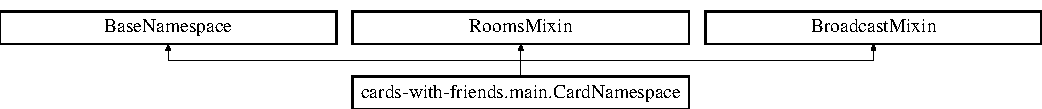
\includegraphics[height=1.464052cm]{classcards-with-friends_1_1main_1_1_card_namespace}
\end{center}
\end{figure}
\subsection*{Public Member Functions}
\begin{DoxyCompactItemize}
\item 
\hypertarget{classcards-with-friends_1_1main_1_1_card_namespace_a3741b80bddf9ab7b94559dcd84dc185e}{def {\bfseries on\-\_\-reconnect}}\label{classcards-with-friends_1_1main_1_1_card_namespace_a3741b80bddf9ab7b94559dcd84dc185e}

\item 
\hypertarget{classcards-with-friends_1_1main_1_1_card_namespace_a77e2af8abc15d48672e6e8e570984d57}{def {\bfseries on\-\_\-card}}\label{classcards-with-friends_1_1main_1_1_card_namespace_a77e2af8abc15d48672e6e8e570984d57}

\item 
\hypertarget{classcards-with-friends_1_1main_1_1_card_namespace_aed7cef092f5eea9a257aebdae7debd4e}{def {\bfseries on\-\_\-bid}}\label{classcards-with-friends_1_1main_1_1_card_namespace_aed7cef092f5eea9a257aebdae7debd4e}

\item 
\hypertarget{classcards-with-friends_1_1main_1_1_card_namespace_a288b1be2c4aaafcef3d7abb6c54cc13a}{def {\bfseries add\-\_\-card}}\label{classcards-with-friends_1_1main_1_1_card_namespace_a288b1be2c4aaafcef3d7abb6c54cc13a}

\item 
\hypertarget{classcards-with-friends_1_1main_1_1_card_namespace_a7f85953a3ee6a2072b1b41e2f589d98c}{def {\bfseries get\-\_\-card}}\label{classcards-with-friends_1_1main_1_1_card_namespace_a7f85953a3ee6a2072b1b41e2f589d98c}

\item 
\hypertarget{classcards-with-friends_1_1main_1_1_card_namespace_aa8f28cbd38b8df0d53a7a0ab44753ba1}{def {\bfseries get\-\_\-bid}}\label{classcards-with-friends_1_1main_1_1_card_namespace_aa8f28cbd38b8df0d53a7a0ab44753ba1}

\item 
\hypertarget{classcards-with-friends_1_1main_1_1_card_namespace_ac92f807282d3b00796af82757bbdef41}{def {\bfseries clear\-\_\-hand}}\label{classcards-with-friends_1_1main_1_1_card_namespace_ac92f807282d3b00796af82757bbdef41}

\item 
\hypertarget{classcards-with-friends_1_1main_1_1_card_namespace_a7fbf1b76d2ae0df496728489d0a128b7}{def {\bfseries remove\-\_\-card}}\label{classcards-with-friends_1_1main_1_1_card_namespace_a7fbf1b76d2ae0df496728489d0a128b7}

\item 
\hypertarget{classcards-with-friends_1_1main_1_1_card_namespace_af498fe88c451173b8360bb4902bebc4f}{def {\bfseries add\-\_\-to\-\_\-trick\-\_\-area}}\label{classcards-with-friends_1_1main_1_1_card_namespace_af498fe88c451173b8360bb4902bebc4f}

\item 
\hypertarget{classcards-with-friends_1_1main_1_1_card_namespace_a3d64d7dda35f80ca14e5c5cf5e6d8119}{def {\bfseries update\-\_\-money}}\label{classcards-with-friends_1_1main_1_1_card_namespace_a3d64d7dda35f80ca14e5c5cf5e6d8119}

\item 
\hypertarget{classcards-with-friends_1_1main_1_1_card_namespace_abdefa7cd21d4a0553186f6592d0f1288}{def {\bfseries update\-\_\-score}}\label{classcards-with-friends_1_1main_1_1_card_namespace_abdefa7cd21d4a0553186f6592d0f1288}

\item 
\hypertarget{classcards-with-friends_1_1main_1_1_card_namespace_ae311e2b7b5cf13cefd02c62727a3a8fc}{def {\bfseries take\-\_\-trick}}\label{classcards-with-friends_1_1main_1_1_card_namespace_ae311e2b7b5cf13cefd02c62727a3a8fc}

\item 
\hypertarget{classcards-with-friends_1_1main_1_1_card_namespace_a0e6c3f5c9b34a5d2a54b7653ed8f8a10}{def {\bfseries clear\-\_\-taken}}\label{classcards-with-friends_1_1main_1_1_card_namespace_a0e6c3f5c9b34a5d2a54b7653ed8f8a10}

\item 
\hypertarget{classcards-with-friends_1_1main_1_1_card_namespace_a6290d8089ecd24be2be78199e2ba4267}{def {\bfseries start\-\_\-turn}}\label{classcards-with-friends_1_1main_1_1_card_namespace_a6290d8089ecd24be2be78199e2ba4267}

\item 
\hypertarget{classcards-with-friends_1_1main_1_1_card_namespace_a21738e86d1d567c5326e7cce192483be}{def {\bfseries end\-\_\-turn}}\label{classcards-with-friends_1_1main_1_1_card_namespace_a21738e86d1d567c5326e7cce192483be}

\item 
\hypertarget{classcards-with-friends_1_1main_1_1_card_namespace_aee69bb5355591bb915c2c4c650824917}{def {\bfseries display\-\_\-message}}\label{classcards-with-friends_1_1main_1_1_card_namespace_aee69bb5355591bb915c2c4c650824917}

\item 
\hypertarget{classcards-with-friends_1_1main_1_1_card_namespace_aa8260bc96e76583841726e8e5d4b6bdd}{def {\bfseries on\-\_\-request\-\_\-room\-\_\-list}}\label{classcards-with-friends_1_1main_1_1_card_namespace_aa8260bc96e76583841726e8e5d4b6bdd}

\item 
\hypertarget{classcards-with-friends_1_1main_1_1_card_namespace_a617d0bb738dbbf8fd826f9318f05ae24}{def {\bfseries update\-\_\-room\-\_\-list}}\label{classcards-with-friends_1_1main_1_1_card_namespace_a617d0bb738dbbf8fd826f9318f05ae24}

\item 
\hypertarget{classcards-with-friends_1_1main_1_1_card_namespace_a53f235205f1ada1ca3740c6c928b767c}{def {\bfseries on\-\_\-create\-\_\-room}}\label{classcards-with-friends_1_1main_1_1_card_namespace_a53f235205f1ada1ca3740c6c928b767c}

\item 
\hypertarget{classcards-with-friends_1_1main_1_1_card_namespace_ae3b139f15f78af1b203401761171ff3b}{def {\bfseries on\-\_\-join}}\label{classcards-with-friends_1_1main_1_1_card_namespace_ae3b139f15f78af1b203401761171ff3b}

\item 
\hypertarget{classcards-with-friends_1_1main_1_1_card_namespace_add17d030e32cfedacf12bbf272b29635}{def {\bfseries on\-\_\-leave}}\label{classcards-with-friends_1_1main_1_1_card_namespace_add17d030e32cfedacf12bbf272b29635}

\item 
\hypertarget{classcards-with-friends_1_1main_1_1_card_namespace_a89dbdc0ba5113019e9b3dfd8f298c026}{def {\bfseries on\-\_\-delete\-\_\-room}}\label{classcards-with-friends_1_1main_1_1_card_namespace_a89dbdc0ba5113019e9b3dfd8f298c026}

\item 
\hypertarget{classcards-with-friends_1_1main_1_1_card_namespace_ae1fa0fdb798cbeec1b68d9b52799e306}{def {\bfseries on\-\_\-start\-\_\-game}}\label{classcards-with-friends_1_1main_1_1_card_namespace_ae1fa0fdb798cbeec1b68d9b52799e306}

\item 
\hypertarget{classcards-with-friends_1_1main_1_1_card_namespace_a4b5eb60a8135ebd793af13eb38dbdf7d}{def {\bfseries on\-\_\-ready\-\_\-game}}\label{classcards-with-friends_1_1main_1_1_card_namespace_a4b5eb60a8135ebd793af13eb38dbdf7d}

\end{DoxyCompactItemize}
\subsection*{Static Public Member Functions}
\begin{DoxyCompactItemize}
\item 
\hypertarget{classcards-with-friends_1_1main_1_1_card_namespace_a614873907f405a35cb1430f7686450d8}{def {\bfseries update\-\_\-all\-\_\-room\-\_\-lists}}\label{classcards-with-friends_1_1main_1_1_card_namespace_a614873907f405a35cb1430f7686450d8}

\end{DoxyCompactItemize}
\subsection*{Public Attributes}
\begin{DoxyCompactItemize}
\item 
\hypertarget{classcards-with-friends_1_1main_1_1_card_namespace_acfafa108ae7d4c75371d7f1ece91dd47}{{\bfseries is\-Host}}\label{classcards-with-friends_1_1main_1_1_card_namespace_acfafa108ae7d4c75371d7f1ece91dd47}

\item 
\hypertarget{classcards-with-friends_1_1main_1_1_card_namespace_abdc84b8283a2d591e4574e33d0606a4e}{{\bfseries nickname}}\label{classcards-with-friends_1_1main_1_1_card_namespace_abdc84b8283a2d591e4574e33d0606a4e}

\item 
\hypertarget{classcards-with-friends_1_1main_1_1_card_namespace_abe7c5d6bfc646a816b4598b87d5a1132}{{\bfseries card}}\label{classcards-with-friends_1_1main_1_1_card_namespace_abe7c5d6bfc646a816b4598b87d5a1132}

\item 
\hypertarget{classcards-with-friends_1_1main_1_1_card_namespace_a6a6f91ae450818aca905d26039e6646c}{{\bfseries bid}}\label{classcards-with-friends_1_1main_1_1_card_namespace_a6a6f91ae450818aca905d26039e6646c}

\end{DoxyCompactItemize}
\subsection*{Static Public Attributes}
\begin{DoxyCompactItemize}
\item 
\hypertarget{classcards-with-friends_1_1main_1_1_card_namespace_a083dcb4c4505532ff93faa66a868fb8d}{tuple {\bfseries manager} = \hyperlink{classcards-with-friends_1_1main_1_1_game_manager}{Game\-Manager}()}\label{classcards-with-friends_1_1main_1_1_card_namespace_a083dcb4c4505532ff93faa66a868fb8d}

\item 
\hypertarget{classcards-with-friends_1_1main_1_1_card_namespace_a3c4e4bc0569cefec5817e2625bb86904}{list {\bfseries rooms} = \mbox{[}$\,$\mbox{]}}\label{classcards-with-friends_1_1main_1_1_card_namespace_a3c4e4bc0569cefec5817e2625bb86904}

\item 
\hypertarget{classcards-with-friends_1_1main_1_1_card_namespace_a3f0ffb585b5f79ddd7a8ca6b047515a2}{dictionary {\bfseries players} = \{\}}\label{classcards-with-friends_1_1main_1_1_card_namespace_a3f0ffb585b5f79ddd7a8ca6b047515a2}

\item 
\hypertarget{classcards-with-friends_1_1main_1_1_card_namespace_a32391e63766cbbe2df5972290b3c564b}{dictionary {\bfseries passwords} = \{\}}\label{classcards-with-friends_1_1main_1_1_card_namespace_a32391e63766cbbe2df5972290b3c564b}

\item 
\hypertarget{classcards-with-friends_1_1main_1_1_card_namespace_afea92ae3214ca41ea335937926537fdb}{{\bfseries my\-\_\-room} = None}\label{classcards-with-friends_1_1main_1_1_card_namespace_afea92ae3214ca41ea335937926537fdb}

\item 
\hypertarget{classcards-with-friends_1_1main_1_1_card_namespace_a3e30c3a845a6fdc206db38e4e237d859}{int {\bfseries is\-Host} = 0}\label{classcards-with-friends_1_1main_1_1_card_namespace_a3e30c3a845a6fdc206db38e4e237d859}

\item 
\hypertarget{classcards-with-friends_1_1main_1_1_card_namespace_a55611ac97e973922a06f1ff813c74745}{string {\bfseries nickname} = \char`\"{}\char`\"{}}\label{classcards-with-friends_1_1main_1_1_card_namespace_a55611ac97e973922a06f1ff813c74745}

\item 
\hypertarget{classcards-with-friends_1_1main_1_1_card_namespace_a79b6d468dae49167cc9b841ee8380310}{{\bfseries ready} = False}\label{classcards-with-friends_1_1main_1_1_card_namespace_a79b6d468dae49167cc9b841ee8380310}

\end{DoxyCompactItemize}


The documentation for this class was generated from the following file\-:\begin{DoxyCompactItemize}
\item 
main.\-py\end{DoxyCompactItemize}

\hypertarget{classcards-with-friends_1_1deck_1_1_deck}{\section{cards-\/with-\/friends.deck.\-Deck Class Reference}
\label{classcards-with-friends_1_1deck_1_1_deck}\index{cards-\/with-\/friends.\-deck.\-Deck@{cards-\/with-\/friends.\-deck.\-Deck}}
}
Inheritance diagram for cards-\/with-\/friends.deck.\-Deck\-:\begin{figure}[H]
\begin{center}
\leavevmode
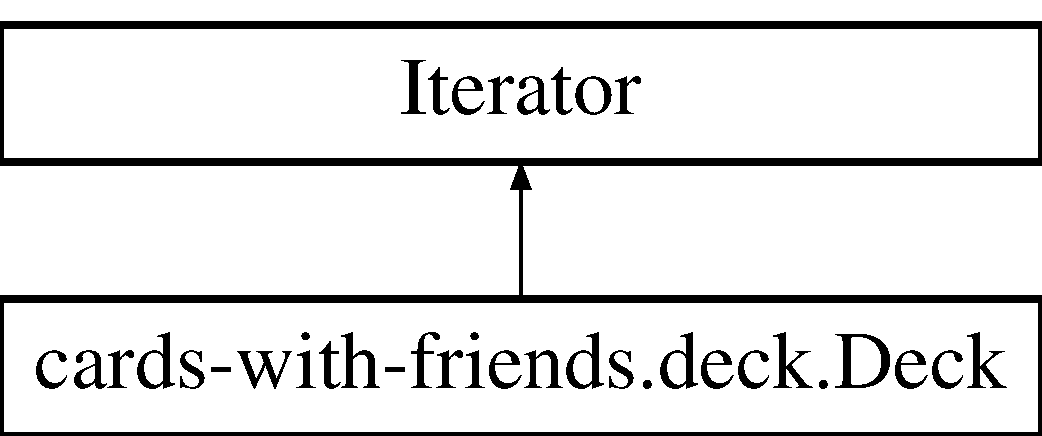
\includegraphics[height=2.000000cm]{classcards-with-friends_1_1deck_1_1_deck}
\end{center}
\end{figure}
\subsection*{Public Member Functions}
\begin{DoxyCompactItemize}
\item 
def \hyperlink{classcards-with-friends_1_1deck_1_1_deck_a4fe6b068257e432ad53061f38f7b41ad}{\-\_\-\-\_\-init\-\_\-\-\_\-}
\item 
\hypertarget{classcards-with-friends_1_1deck_1_1_deck_aba07c6e99b729b42a1b1e664272d4025}{def {\bfseries \-\_\-\-\_\-len\-\_\-\-\_\-}}\label{classcards-with-friends_1_1deck_1_1_deck_aba07c6e99b729b42a1b1e664272d4025}

\item 
\hypertarget{classcards-with-friends_1_1deck_1_1_deck_a05499246dcf44b6a0e6b868faa1b7d53}{def {\bfseries \-\_\-\-\_\-nonzero\-\_\-\-\_\-}}\label{classcards-with-friends_1_1deck_1_1_deck_a05499246dcf44b6a0e6b868faa1b7d53}

\item 
\hypertarget{classcards-with-friends_1_1deck_1_1_deck_a762d0eaa69201df45fa907d22caee2b5}{def {\bfseries \-\_\-\-\_\-repr\-\_\-\-\_\-}}\label{classcards-with-friends_1_1deck_1_1_deck_a762d0eaa69201df45fa907d22caee2b5}

\item 
def \hyperlink{classcards-with-friends_1_1deck_1_1_deck_a805f4390141a790fb0b8ac498e38b727}{fromjson}
\item 
\hypertarget{classcards-with-friends_1_1deck_1_1_deck_af5b795d0f0b9d9ec9e1bcdb718514b2f}{def {\bfseries next}}\label{classcards-with-friends_1_1deck_1_1_deck_af5b795d0f0b9d9ec9e1bcdb718514b2f}

\item 
def \hyperlink{classcards-with-friends_1_1deck_1_1_deck_a3831e8133c28c3ac53cc34285bdd4403}{Draw}
\item 
def \hyperlink{classcards-with-friends_1_1deck_1_1_deck_abbf374196d0f5f94c38dfbadeb9a8893}{Find\-And\-Remove\-Card}
\item 
\hypertarget{classcards-with-friends_1_1deck_1_1_deck_aa167404db0fe4cbe2ddf80a31c949c03}{def {\bfseries Get\-Back\-Image}}\label{classcards-with-friends_1_1deck_1_1_deck_aa167404db0fe4cbe2ddf80a31c949c03}

\item 
def \hyperlink{classcards-with-friends_1_1deck_1_1_deck_a0f17fe6567d06d5a653658f3b8c77571}{Shuffle}
\item 
\hypertarget{classcards-with-friends_1_1deck_1_1_deck_a5dd5e42df80bd51061868eecf47da588}{def {\bfseries Write\-To\-File}}\label{classcards-with-friends_1_1deck_1_1_deck_a5dd5e42df80bd51061868eecf47da588}

\item 
\hypertarget{classcards-with-friends_1_1deck_1_1_deck_a9fb70e1293a51e1ef2935ade659a9d6c}{def {\bfseries back\-\_\-image\-\_\-loc}}\label{classcards-with-friends_1_1deck_1_1_deck_a9fb70e1293a51e1ef2935ade659a9d6c}

\item 
\hypertarget{classcards-with-friends_1_1deck_1_1_deck_ac2c367963068fed1f02173c5c40b5dcf}{def {\bfseries long\-\_\-name}}\label{classcards-with-friends_1_1deck_1_1_deck_ac2c367963068fed1f02173c5c40b5dcf}

\item 
\hypertarget{classcards-with-friends_1_1deck_1_1_deck_ad5b3f496588fb6367f8299ef5feec2d7}{def {\bfseries name}}\label{classcards-with-friends_1_1deck_1_1_deck_ad5b3f496588fb6367f8299ef5feec2d7}

\end{DoxyCompactItemize}


\subsection{Detailed Description}
\begin{DoxyVerb}A deck of playing cards.\end{DoxyVerb}
 

\subsection{Constructor \& Destructor Documentation}
\hypertarget{classcards-with-friends_1_1deck_1_1_deck_a4fe6b068257e432ad53061f38f7b41ad}{\index{cards-\/with-\/friends\-::deck\-::\-Deck@{cards-\/with-\/friends\-::deck\-::\-Deck}!\-\_\-\-\_\-init\-\_\-\-\_\-@{\-\_\-\-\_\-init\-\_\-\-\_\-}}
\index{\-\_\-\-\_\-init\-\_\-\-\_\-@{\-\_\-\-\_\-init\-\_\-\-\_\-}!cards-with-friends::deck::Deck@{cards-\/with-\/friends\-::deck\-::\-Deck}}
\subsubsection[{\-\_\-\-\_\-init\-\_\-\-\_\-}]{\setlength{\rightskip}{0pt plus 5cm}def cards-\/with-\/friends.\-deck.\-Deck.\-\_\-\-\_\-init\-\_\-\-\_\- (
\begin{DoxyParamCaption}
\item[{}]{self, }
\item[{}]{name, }
\item[{}]{long\-\_\-name, }
\item[{}]{back\-\_\-image\-\_\-loc}
\end{DoxyParamCaption}
)}}\label{classcards-with-friends_1_1deck_1_1_deck_a4fe6b068257e432ad53061f38f7b41ad}
\begin{DoxyVerb}Create a deck from a list of cards.

Args:
  name: A unique identifier for the deck.
  long_name: The long name of the deck.
  back_image_loc: The image location for the back of each card.
\end{DoxyVerb}
 

\subsection{Member Function Documentation}
\hypertarget{classcards-with-friends_1_1deck_1_1_deck_a3831e8133c28c3ac53cc34285bdd4403}{\index{cards-\/with-\/friends\-::deck\-::\-Deck@{cards-\/with-\/friends\-::deck\-::\-Deck}!Draw@{Draw}}
\index{Draw@{Draw}!cards-with-friends::deck::Deck@{cards-\/with-\/friends\-::deck\-::\-Deck}}
\subsubsection[{Draw}]{\setlength{\rightskip}{0pt plus 5cm}def cards-\/with-\/friends.\-deck.\-Deck.\-Draw (
\begin{DoxyParamCaption}
\item[{}]{self, }
\item[{}]{num\-\_\-cards = {\ttfamily 1}}
\end{DoxyParamCaption}
)}}\label{classcards-with-friends_1_1deck_1_1_deck_a3831e8133c28c3ac53cc34285bdd4403}
\begin{DoxyVerb}Remove and return the top num_card cards (default 1) from the deck as a list.\end{DoxyVerb}
 \hypertarget{classcards-with-friends_1_1deck_1_1_deck_abbf374196d0f5f94c38dfbadeb9a8893}{\index{cards-\/with-\/friends\-::deck\-::\-Deck@{cards-\/with-\/friends\-::deck\-::\-Deck}!Find\-And\-Remove\-Card@{Find\-And\-Remove\-Card}}
\index{Find\-And\-Remove\-Card@{Find\-And\-Remove\-Card}!cards-with-friends::deck::Deck@{cards-\/with-\/friends\-::deck\-::\-Deck}}
\subsubsection[{Find\-And\-Remove\-Card}]{\setlength{\rightskip}{0pt plus 5cm}def cards-\/with-\/friends.\-deck.\-Deck.\-Find\-And\-Remove\-Card (
\begin{DoxyParamCaption}
\item[{}]{self, }
\item[{}]{props}
\end{DoxyParamCaption}
)}}\label{classcards-with-friends_1_1deck_1_1_deck_abbf374196d0f5f94c38dfbadeb9a8893}
\begin{DoxyVerb}Find a card given its properties and remove the first match from the deck.\end{DoxyVerb}
 \hypertarget{classcards-with-friends_1_1deck_1_1_deck_a805f4390141a790fb0b8ac498e38b727}{\index{cards-\/with-\/friends\-::deck\-::\-Deck@{cards-\/with-\/friends\-::deck\-::\-Deck}!fromjson@{fromjson}}
\index{fromjson@{fromjson}!cards-with-friends::deck::Deck@{cards-\/with-\/friends\-::deck\-::\-Deck}}
\subsubsection[{fromjson}]{\setlength{\rightskip}{0pt plus 5cm}def cards-\/with-\/friends.\-deck.\-Deck.\-fromjson (
\begin{DoxyParamCaption}
\item[{}]{cls, }
\item[{}]{filepath}
\end{DoxyParamCaption}
)}}\label{classcards-with-friends_1_1deck_1_1_deck_a805f4390141a790fb0b8ac498e38b727}
\begin{DoxyVerb}Create a deck from a JSON file.

The file format is explained elsewhere.
\end{DoxyVerb}
 \hypertarget{classcards-with-friends_1_1deck_1_1_deck_a0f17fe6567d06d5a653658f3b8c77571}{\index{cards-\/with-\/friends\-::deck\-::\-Deck@{cards-\/with-\/friends\-::deck\-::\-Deck}!Shuffle@{Shuffle}}
\index{Shuffle@{Shuffle}!cards-with-friends::deck::Deck@{cards-\/with-\/friends\-::deck\-::\-Deck}}
\subsubsection[{Shuffle}]{\setlength{\rightskip}{0pt plus 5cm}def cards-\/with-\/friends.\-deck.\-Deck.\-Shuffle (
\begin{DoxyParamCaption}
\item[{}]{self, }
\item[{}]{reset = {\ttfamily True}}
\end{DoxyParamCaption}
)}}\label{classcards-with-friends_1_1deck_1_1_deck_a0f17fe6567d06d5a653658f3b8c77571}
\begin{DoxyVerb}Shuffle the deck.\end{DoxyVerb}
 

The documentation for this class was generated from the following file\-:\begin{DoxyCompactItemize}
\item 
deck.\-py\end{DoxyCompactItemize}

\hypertarget{classcards-with-friends_1_1game_1_1_game}{\section{cards-\/with-\/friends.game.\-Game Class Reference}
\label{classcards-with-friends_1_1game_1_1_game}\index{cards-\/with-\/friends.\-game.\-Game@{cards-\/with-\/friends.\-game.\-Game}}
}
Inheritance diagram for cards-\/with-\/friends.game.\-Game\-:\begin{figure}[H]
\begin{center}
\leavevmode
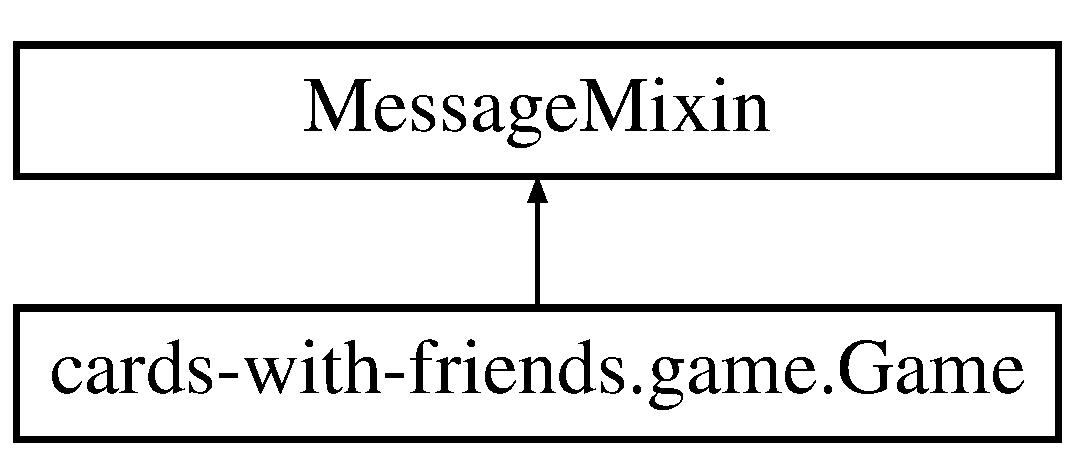
\includegraphics[height=2.000000cm]{classcards-with-friends_1_1game_1_1_game}
\end{center}
\end{figure}
\subsection*{Public Member Functions}
\begin{DoxyCompactItemize}
\item 
def \hyperlink{classcards-with-friends_1_1game_1_1_game_a11c7ae2e00ff8af5a510ebfc14d43635}{\-\_\-\-\_\-init\-\_\-\-\_\-}
\item 
\hypertarget{classcards-with-friends_1_1game_1_1_game_ab364e816fad8ae7537af4339ca2ef593}{def {\bfseries \-\_\-\-\_\-getattribute\-\_\-\-\_\-}}\label{classcards-with-friends_1_1game_1_1_game_ab364e816fad8ae7537af4339ca2ef593}

\item 
\hypertarget{classcards-with-friends_1_1game_1_1_game_ab93a7b3660cdb7e2383206610bc6a6a3}{def {\bfseries \-\_\-\-\_\-repr\-\_\-\-\_\-}}\label{classcards-with-friends_1_1game_1_1_game_ab93a7b3660cdb7e2383206610bc6a6a3}

\item 
\hypertarget{classcards-with-friends_1_1game_1_1_game_a06719d07da4776303f5dd7b50ca4bb22}{def {\bfseries \-\_\-\-\_\-setattr\-\_\-\-\_\-}}\label{classcards-with-friends_1_1game_1_1_game_a06719d07da4776303f5dd7b50ca4bb22}

\item 
def \hyperlink{classcards-with-friends_1_1game_1_1_game_a44a3fcdf59ea4be488aac3db7a01a91d}{Get\-Player\-By\-Index}
\item 
def \hyperlink{classcards-with-friends_1_1game_1_1_game_a5df2b7942c2b2707cd766dd340e5e513}{Get\-Player\-By\-Name}
\item 
def \hyperlink{classcards-with-friends_1_1game_1_1_game_acf2a8ec5e9625ecc732a25c4855d2934}{Get\-Player\-Index}
\item 
def \hyperlink{classcards-with-friends_1_1game_1_1_game_a65be6ddba2240807dca1edc0ef7974d2}{Reset\-Players}
\item 
\hypertarget{classcards-with-friends_1_1game_1_1_game_a6259d61238d30de3629e369c835a0bba}{def {\bfseries dealer}}\label{classcards-with-friends_1_1game_1_1_game_a6259d61238d30de3629e369c835a0bba}

\item 
\hypertarget{classcards-with-friends_1_1game_1_1_game_a6259d61238d30de3629e369c835a0bba}{def {\bfseries dealer}}\label{classcards-with-friends_1_1game_1_1_game_a6259d61238d30de3629e369c835a0bba}

\item 
\hypertarget{classcards-with-friends_1_1game_1_1_game_ab49a2d8d555152ad6b3bd70f269457d7}{def {\bfseries deck}}\label{classcards-with-friends_1_1game_1_1_game_ab49a2d8d555152ad6b3bd70f269457d7}

\item 
\hypertarget{classcards-with-friends_1_1game_1_1_game_a17b4af32e7b279e0e763cee4509e5aff}{def {\bfseries id}}\label{classcards-with-friends_1_1game_1_1_game_a17b4af32e7b279e0e763cee4509e5aff}

\item 
\hypertarget{classcards-with-friends_1_1game_1_1_game_ab4c6673f094b22423d0cbb68a310881d}{def {\bfseries num\-\_\-players}}\label{classcards-with-friends_1_1game_1_1_game_ab4c6673f094b22423d0cbb68a310881d}

\item 
\hypertarget{classcards-with-friends_1_1game_1_1_game_aee0fbc62f41d87a8c14e96c2aef08c31}{def {\bfseries players}}\label{classcards-with-friends_1_1game_1_1_game_aee0fbc62f41d87a8c14e96c2aef08c31}

\item 
\hypertarget{classcards-with-friends_1_1game_1_1_game_a12a542866da6a5052ef1731e7666fd03}{def {\bfseries players\-\_\-by\-\_\-name}}\label{classcards-with-friends_1_1game_1_1_game_a12a542866da6a5052ef1731e7666fd03}

\end{DoxyCompactItemize}


\subsection{Detailed Description}
\begin{DoxyVerb}A card game.\end{DoxyVerb}
 

\subsection{Constructor \& Destructor Documentation}
\hypertarget{classcards-with-friends_1_1game_1_1_game_a11c7ae2e00ff8af5a510ebfc14d43635}{\index{cards-\/with-\/friends\-::game\-::\-Game@{cards-\/with-\/friends\-::game\-::\-Game}!\-\_\-\-\_\-init\-\_\-\-\_\-@{\-\_\-\-\_\-init\-\_\-\-\_\-}}
\index{\-\_\-\-\_\-init\-\_\-\-\_\-@{\-\_\-\-\_\-init\-\_\-\-\_\-}!cards-with-friends::game::Game@{cards-\/with-\/friends\-::game\-::\-Game}}
\subsubsection[{\-\_\-\-\_\-init\-\_\-\-\_\-}]{\setlength{\rightskip}{0pt plus 5cm}def cards-\/with-\/friends.\-game.\-Game.\-\_\-\-\_\-init\-\_\-\-\_\- (
\begin{DoxyParamCaption}
\item[{}]{self, }
\item[{}]{players, }
\item[{}]{deck}
\end{DoxyParamCaption}
)}}\label{classcards-with-friends_1_1game_1_1_game_a11c7ae2e00ff8af5a510ebfc14d43635}
\begin{DoxyVerb}Constructor.

Args:
  players: A list of Player objects.
  deck: The name of the deck for this game.
\end{DoxyVerb}
 

\subsection{Member Function Documentation}
\hypertarget{classcards-with-friends_1_1game_1_1_game_a44a3fcdf59ea4be488aac3db7a01a91d}{\index{cards-\/with-\/friends\-::game\-::\-Game@{cards-\/with-\/friends\-::game\-::\-Game}!Get\-Player\-By\-Index@{Get\-Player\-By\-Index}}
\index{Get\-Player\-By\-Index@{Get\-Player\-By\-Index}!cards-with-friends::game::Game@{cards-\/with-\/friends\-::game\-::\-Game}}
\subsubsection[{Get\-Player\-By\-Index}]{\setlength{\rightskip}{0pt plus 5cm}def cards-\/with-\/friends.\-game.\-Game.\-Get\-Player\-By\-Index (
\begin{DoxyParamCaption}
\item[{}]{self, }
\item[{}]{index}
\end{DoxyParamCaption}
)}}\label{classcards-with-friends_1_1game_1_1_game_a44a3fcdf59ea4be488aac3db7a01a91d}
\begin{DoxyVerb}Get a player in the list of players at the specified index (modulo the number of players)\end{DoxyVerb}
 \hypertarget{classcards-with-friends_1_1game_1_1_game_a5df2b7942c2b2707cd766dd340e5e513}{\index{cards-\/with-\/friends\-::game\-::\-Game@{cards-\/with-\/friends\-::game\-::\-Game}!Get\-Player\-By\-Name@{Get\-Player\-By\-Name}}
\index{Get\-Player\-By\-Name@{Get\-Player\-By\-Name}!cards-with-friends::game::Game@{cards-\/with-\/friends\-::game\-::\-Game}}
\subsubsection[{Get\-Player\-By\-Name}]{\setlength{\rightskip}{0pt plus 5cm}def cards-\/with-\/friends.\-game.\-Game.\-Get\-Player\-By\-Name (
\begin{DoxyParamCaption}
\item[{}]{self, }
\item[{}]{name}
\end{DoxyParamCaption}
)}}\label{classcards-with-friends_1_1game_1_1_game_a5df2b7942c2b2707cd766dd340e5e513}
\begin{DoxyVerb}Get a player by their name. If the player cannot be found, raise an error.\end{DoxyVerb}
 \hypertarget{classcards-with-friends_1_1game_1_1_game_acf2a8ec5e9625ecc732a25c4855d2934}{\index{cards-\/with-\/friends\-::game\-::\-Game@{cards-\/with-\/friends\-::game\-::\-Game}!Get\-Player\-Index@{Get\-Player\-Index}}
\index{Get\-Player\-Index@{Get\-Player\-Index}!cards-with-friends::game::Game@{cards-\/with-\/friends\-::game\-::\-Game}}
\subsubsection[{Get\-Player\-Index}]{\setlength{\rightskip}{0pt plus 5cm}def cards-\/with-\/friends.\-game.\-Game.\-Get\-Player\-Index (
\begin{DoxyParamCaption}
\item[{}]{self, }
\item[{}]{player}
\end{DoxyParamCaption}
)}}\label{classcards-with-friends_1_1game_1_1_game_acf2a8ec5e9625ecc732a25c4855d2934}
\begin{DoxyVerb}Get the index of a player given an instance of a player. If the player cannot be found, raise an error.\end{DoxyVerb}
 \hypertarget{classcards-with-friends_1_1game_1_1_game_a65be6ddba2240807dca1edc0ef7974d2}{\index{cards-\/with-\/friends\-::game\-::\-Game@{cards-\/with-\/friends\-::game\-::\-Game}!Reset\-Players@{Reset\-Players}}
\index{Reset\-Players@{Reset\-Players}!cards-with-friends::game::Game@{cards-\/with-\/friends\-::game\-::\-Game}}
\subsubsection[{Reset\-Players}]{\setlength{\rightskip}{0pt plus 5cm}def cards-\/with-\/friends.\-game.\-Game.\-Reset\-Players (
\begin{DoxyParamCaption}
\item[{}]{self, }
\item[{}]{score = {\ttfamily None}}
\end{DoxyParamCaption}
)}}\label{classcards-with-friends_1_1game_1_1_game_a65be6ddba2240807dca1edc0ef7974d2}
\begin{DoxyVerb}Reset the state of every player: clear the hands and cards taken, and set the score of every player to the specified score.\end{DoxyVerb}
 

The documentation for this class was generated from the following file\-:\begin{DoxyCompactItemize}
\item 
game.\-py\end{DoxyCompactItemize}

\hypertarget{classcards-with-friends_1_1main_1_1_game_manager}{\section{cards-\/with-\/friends.main.\-Game\-Manager Class Reference}
\label{classcards-with-friends_1_1main_1_1_game_manager}\index{cards-\/with-\/friends.\-main.\-Game\-Manager@{cards-\/with-\/friends.\-main.\-Game\-Manager}}
}


C\-L\-A\-S\-S\-E\-S.  


Inheritance diagram for cards-\/with-\/friends.main.\-Game\-Manager\-:\begin{figure}[H]
\begin{center}
\leavevmode
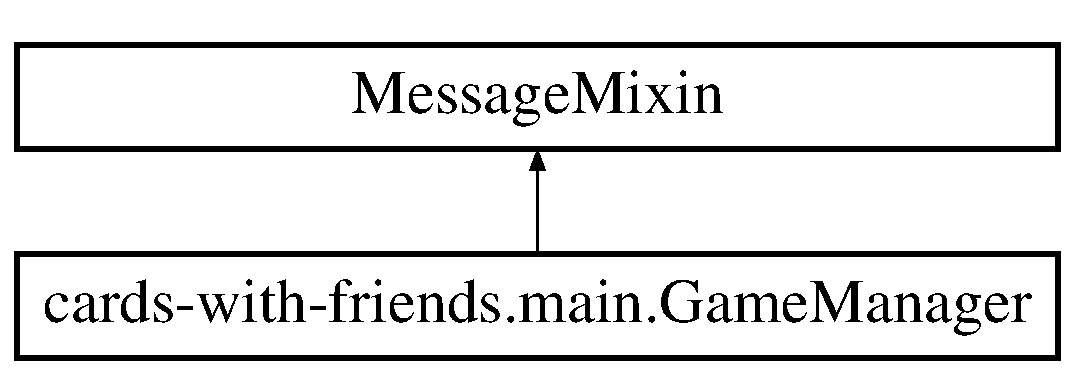
\includegraphics[height=2.000000cm]{classcards-with-friends_1_1main_1_1_game_manager}
\end{center}
\end{figure}
\subsection*{Public Member Functions}
\begin{DoxyCompactItemize}
\item 
def \hyperlink{classcards-with-friends_1_1main_1_1_game_manager_a8bd05763ca0177454d4b0620a739b3ac}{Create\-Game}
\item 
def \hyperlink{classcards-with-friends_1_1main_1_1_game_manager_aa9a818023bacf5cbf1a6862e6c53d840}{Delete\-Game}
\item 
def \hyperlink{classcards-with-friends_1_1main_1_1_game_manager_ac6bc592b254796ea9e4376285401d688}{Start\-Game}
\end{DoxyCompactItemize}
\subsection*{Static Public Attributes}
\begin{DoxyCompactItemize}
\item 
\hypertarget{classcards-with-friends_1_1main_1_1_game_manager_ac4794e33676e2c740874d72a2174b7df}{dictionary {\bfseries games} = \{\}}\label{classcards-with-friends_1_1main_1_1_game_manager_ac4794e33676e2c740874d72a2174b7df}

\item 
\hypertarget{classcards-with-friends_1_1main_1_1_game_manager_a81dcc2d29e24e67f3f8e03a0a6e7d817}{dictionary {\bfseries players} = \{\}}\label{classcards-with-friends_1_1main_1_1_game_manager_a81dcc2d29e24e67f3f8e03a0a6e7d817}

\item 
\hypertarget{classcards-with-friends_1_1main_1_1_game_manager_ac6a25f45208944621318ba8aa179a359}{tuple {\bfseries in\-\_\-room} = weakref.\-Weak\-Value\-Dictionary()}\label{classcards-with-friends_1_1main_1_1_game_manager_ac6a25f45208944621318ba8aa179a359}

\end{DoxyCompactItemize}


\subsection{Detailed Description}
C\-L\-A\-S\-S\-E\-S. 

\begin{DoxyVerb}Manages games and scores.\end{DoxyVerb}
 

\subsection{Member Function Documentation}
\hypertarget{classcards-with-friends_1_1main_1_1_game_manager_a8bd05763ca0177454d4b0620a739b3ac}{\index{cards-\/with-\/friends\-::main\-::\-Game\-Manager@{cards-\/with-\/friends\-::main\-::\-Game\-Manager}!Create\-Game@{Create\-Game}}
\index{Create\-Game@{Create\-Game}!cards-with-friends::main::GameManager@{cards-\/with-\/friends\-::main\-::\-Game\-Manager}}
\subsubsection[{Create\-Game}]{\setlength{\rightskip}{0pt plus 5cm}def cards-\/with-\/friends.\-main.\-Game\-Manager.\-Create\-Game (
\begin{DoxyParamCaption}
\item[{}]{self, }
\item[{}]{game\-\_\-type, }
\item[{}]{players}
\end{DoxyParamCaption}
)}}\label{classcards-with-friends_1_1main_1_1_game_manager_a8bd05763ca0177454d4b0620a739b3ac}
\begin{DoxyVerb}Create a new game.\end{DoxyVerb}
 \hypertarget{classcards-with-friends_1_1main_1_1_game_manager_aa9a818023bacf5cbf1a6862e6c53d840}{\index{cards-\/with-\/friends\-::main\-::\-Game\-Manager@{cards-\/with-\/friends\-::main\-::\-Game\-Manager}!Delete\-Game@{Delete\-Game}}
\index{Delete\-Game@{Delete\-Game}!cards-with-friends::main::GameManager@{cards-\/with-\/friends\-::main\-::\-Game\-Manager}}
\subsubsection[{Delete\-Game}]{\setlength{\rightskip}{0pt plus 5cm}def cards-\/with-\/friends.\-main.\-Game\-Manager.\-Delete\-Game (
\begin{DoxyParamCaption}
\item[{}]{self, }
\item[{}]{game\-\_\-id}
\end{DoxyParamCaption}
)}}\label{classcards-with-friends_1_1main_1_1_game_manager_aa9a818023bacf5cbf1a6862e6c53d840}
\begin{DoxyVerb}Delete a previously-created game.\end{DoxyVerb}
 \hypertarget{classcards-with-friends_1_1main_1_1_game_manager_ac6bc592b254796ea9e4376285401d688}{\index{cards-\/with-\/friends\-::main\-::\-Game\-Manager@{cards-\/with-\/friends\-::main\-::\-Game\-Manager}!Start\-Game@{Start\-Game}}
\index{Start\-Game@{Start\-Game}!cards-with-friends::main::GameManager@{cards-\/with-\/friends\-::main\-::\-Game\-Manager}}
\subsubsection[{Start\-Game}]{\setlength{\rightskip}{0pt plus 5cm}def cards-\/with-\/friends.\-main.\-Game\-Manager.\-Start\-Game (
\begin{DoxyParamCaption}
\item[{}]{self, }
\item[{}]{game\-\_\-id}
\end{DoxyParamCaption}
)}}\label{classcards-with-friends_1_1main_1_1_game_manager_ac6bc592b254796ea9e4376285401d688}
\begin{DoxyVerb}Start a previously-created game.\end{DoxyVerb}
 

The documentation for this class was generated from the following file\-:\begin{DoxyCompactItemize}
\item 
main.\-py\end{DoxyCompactItemize}

\hypertarget{classcards-with-friends_1_1games_1_1hearts_1_1_hearts}{\section{cards-\/with-\/friends.games.\-hearts.\-Hearts Class Reference}
\label{classcards-with-friends_1_1games_1_1hearts_1_1_hearts}\index{cards-\/with-\/friends.\-games.\-hearts.\-Hearts@{cards-\/with-\/friends.\-games.\-hearts.\-Hearts}}
}
Inheritance diagram for cards-\/with-\/friends.games.\-hearts.\-Hearts\-:\begin{figure}[H]
\begin{center}
\leavevmode
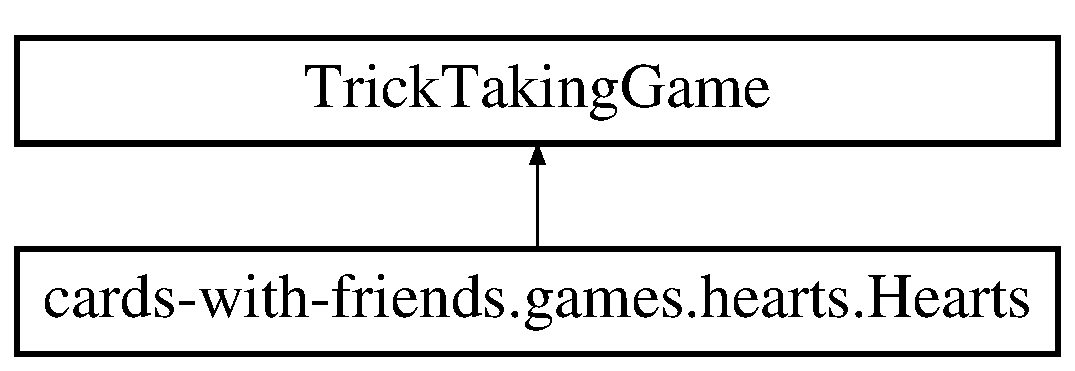
\includegraphics[height=2.000000cm]{classcards-with-friends_1_1games_1_1hearts_1_1_hearts}
\end{center}
\end{figure}
\subsection*{Public Member Functions}
\begin{DoxyCompactItemize}
\item 
\hypertarget{classcards-with-friends_1_1games_1_1hearts_1_1_hearts_a936f6d5d7717c76980b709e0d575c80c}{def {\bfseries \-\_\-\-\_\-init\-\_\-\-\_\-}}\label{classcards-with-friends_1_1games_1_1hearts_1_1_hearts_a936f6d5d7717c76980b709e0d575c80c}

\item 
def \hyperlink{classcards-with-friends_1_1games_1_1hearts_1_1_hearts_aaf67a22977dd621ac3a21663f5702563}{Get\-Card\-Value}
\item 
def \hyperlink{classcards-with-friends_1_1games_1_1hearts_1_1_hearts_ac2cd6b81283c961c434ccea4a6e22889}{Play\-Game}
\item 
def \hyperlink{classcards-with-friends_1_1games_1_1hearts_1_1_hearts_a456f051fffc1e97b24c99bcd3573eda9}{Reset\-Game}
\end{DoxyCompactItemize}
\subsection*{Public Attributes}
\begin{DoxyCompactItemize}
\item 
\hypertarget{classcards-with-friends_1_1games_1_1hearts_1_1_hearts_a30da649bd6eafe45c045e30032922b01}{{\bfseries num\-\_\-players}}\label{classcards-with-friends_1_1games_1_1hearts_1_1_hearts_a30da649bd6eafe45c045e30032922b01}

\item 
\hypertarget{classcards-with-friends_1_1games_1_1hearts_1_1_hearts_ac0dc4138454e9f661e183bd1e816f8e7}{{\bfseries lead}}\label{classcards-with-friends_1_1games_1_1hearts_1_1_hearts_ac0dc4138454e9f661e183bd1e816f8e7}

\item 
\hypertarget{classcards-with-friends_1_1games_1_1hearts_1_1_hearts_a334b803060353eadafeccd821ef19d07}{{\bfseries cards\-\_\-played}}\label{classcards-with-friends_1_1games_1_1hearts_1_1_hearts_a334b803060353eadafeccd821ef19d07}

\item 
\hypertarget{classcards-with-friends_1_1games_1_1hearts_1_1_hearts_a05e0e2f500277376a9bce951c6afffbb}{{\bfseries trick\-\_\-num}}\label{classcards-with-friends_1_1games_1_1hearts_1_1_hearts_a05e0e2f500277376a9bce951c6afffbb}

\item 
\hypertarget{classcards-with-friends_1_1games_1_1hearts_1_1_hearts_a857741e4ede3fc25c2d431b25f9e0a95}{{\bfseries hearts\-\_\-broken}}\label{classcards-with-friends_1_1games_1_1hearts_1_1_hearts_a857741e4ede3fc25c2d431b25f9e0a95}

\end{DoxyCompactItemize}


\subsection{Detailed Description}
\begin{DoxyVerb}The Hearts card game.\end{DoxyVerb}
 

\subsection{Member Function Documentation}
\hypertarget{classcards-with-friends_1_1games_1_1hearts_1_1_hearts_aaf67a22977dd621ac3a21663f5702563}{\index{cards-\/with-\/friends\-::games\-::hearts\-::\-Hearts@{cards-\/with-\/friends\-::games\-::hearts\-::\-Hearts}!Get\-Card\-Value@{Get\-Card\-Value}}
\index{Get\-Card\-Value@{Get\-Card\-Value}!cards-with-friends::games::hearts::Hearts@{cards-\/with-\/friends\-::games\-::hearts\-::\-Hearts}}
\subsubsection[{Get\-Card\-Value}]{\setlength{\rightskip}{0pt plus 5cm}def cards-\/with-\/friends.\-games.\-hearts.\-Hearts.\-Get\-Card\-Value (
\begin{DoxyParamCaption}
\item[{}]{cls, }
\item[{}]{card}
\end{DoxyParamCaption}
)}}\label{classcards-with-friends_1_1games_1_1hearts_1_1_hearts_aaf67a22977dd621ac3a21663f5702563}
\begin{DoxyVerb}Return the value of a card as prescribed by this game.\end{DoxyVerb}
 \hypertarget{classcards-with-friends_1_1games_1_1hearts_1_1_hearts_ac2cd6b81283c961c434ccea4a6e22889}{\index{cards-\/with-\/friends\-::games\-::hearts\-::\-Hearts@{cards-\/with-\/friends\-::games\-::hearts\-::\-Hearts}!Play\-Game@{Play\-Game}}
\index{Play\-Game@{Play\-Game}!cards-with-friends::games::hearts::Hearts@{cards-\/with-\/friends\-::games\-::hearts\-::\-Hearts}}
\subsubsection[{Play\-Game}]{\setlength{\rightskip}{0pt plus 5cm}def cards-\/with-\/friends.\-games.\-hearts.\-Hearts.\-Play\-Game (
\begin{DoxyParamCaption}
\item[{}]{self}
\end{DoxyParamCaption}
)}}\label{classcards-with-friends_1_1games_1_1hearts_1_1_hearts_ac2cd6b81283c961c434ccea4a6e22889}
\begin{DoxyVerb}Play the game.\end{DoxyVerb}
 \hypertarget{classcards-with-friends_1_1games_1_1hearts_1_1_hearts_a456f051fffc1e97b24c99bcd3573eda9}{\index{cards-\/with-\/friends\-::games\-::hearts\-::\-Hearts@{cards-\/with-\/friends\-::games\-::hearts\-::\-Hearts}!Reset\-Game@{Reset\-Game}}
\index{Reset\-Game@{Reset\-Game}!cards-with-friends::games::hearts::Hearts@{cards-\/with-\/friends\-::games\-::hearts\-::\-Hearts}}
\subsubsection[{Reset\-Game}]{\setlength{\rightskip}{0pt plus 5cm}def cards-\/with-\/friends.\-games.\-hearts.\-Hearts.\-Reset\-Game (
\begin{DoxyParamCaption}
\item[{}]{self}
\end{DoxyParamCaption}
)}}\label{classcards-with-friends_1_1games_1_1hearts_1_1_hearts_a456f051fffc1e97b24c99bcd3573eda9}
\begin{DoxyVerb}Reset the entire game state.\end{DoxyVerb}
 

The documentation for this class was generated from the following file\-:\begin{DoxyCompactItemize}
\item 
games/hearts.\-py\end{DoxyCompactItemize}

\hypertarget{classcards-with-friends_1_1games_1_1highest__card_1_1_highest_card}{\section{cards-\/with-\/friends.games.\-highest\-\_\-card.\-Highest\-Card Class Reference}
\label{classcards-with-friends_1_1games_1_1highest__card_1_1_highest_card}\index{cards-\/with-\/friends.\-games.\-highest\-\_\-card.\-Highest\-Card@{cards-\/with-\/friends.\-games.\-highest\-\_\-card.\-Highest\-Card}}
}
Inheritance diagram for cards-\/with-\/friends.games.\-highest\-\_\-card.\-Highest\-Card\-:\begin{figure}[H]
\begin{center}
\leavevmode
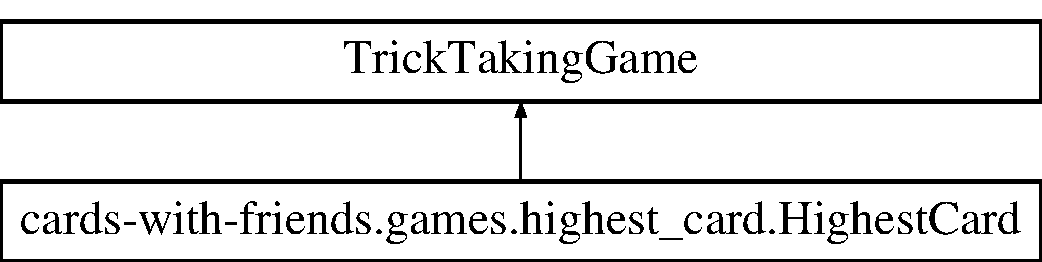
\includegraphics[height=2.000000cm]{classcards-with-friends_1_1games_1_1highest__card_1_1_highest_card}
\end{center}
\end{figure}
\subsection*{Public Member Functions}
\begin{DoxyCompactItemize}
\item 
\hypertarget{classcards-with-friends_1_1games_1_1highest__card_1_1_highest_card_a76637fdd046d57ca7304f94a7338130e}{def {\bfseries \-\_\-\-\_\-init\-\_\-\-\_\-}}\label{classcards-with-friends_1_1games_1_1highest__card_1_1_highest_card_a76637fdd046d57ca7304f94a7338130e}

\item 
def \hyperlink{classcards-with-friends_1_1games_1_1highest__card_1_1_highest_card_a791c4305e07baaa67c67d612ac39648d}{Play\-Game}
\item 
def \hyperlink{classcards-with-friends_1_1games_1_1highest__card_1_1_highest_card_ab6d86edce4aabd740bae250165bb8af9}{Reset\-Game}
\end{DoxyCompactItemize}
\subsection*{Public Attributes}
\begin{DoxyCompactItemize}
\item 
\hypertarget{classcards-with-friends_1_1games_1_1highest__card_1_1_highest_card_ab6be2dc24b7fc75d12acacf8295e0d9f}{{\bfseries lead}}\label{classcards-with-friends_1_1games_1_1highest__card_1_1_highest_card_ab6be2dc24b7fc75d12acacf8295e0d9f}

\item 
\hypertarget{classcards-with-friends_1_1games_1_1highest__card_1_1_highest_card_acf06e3e873edd041e5d5c80a2720a589}{{\bfseries cards\-\_\-played}}\label{classcards-with-friends_1_1games_1_1highest__card_1_1_highest_card_acf06e3e873edd041e5d5c80a2720a589}

\end{DoxyCompactItemize}


\subsection{Detailed Description}
\begin{DoxyVerb}The Highest Card card game.\end{DoxyVerb}
 

\subsection{Member Function Documentation}
\hypertarget{classcards-with-friends_1_1games_1_1highest__card_1_1_highest_card_a791c4305e07baaa67c67d612ac39648d}{\index{cards-\/with-\/friends\-::games\-::highest\-\_\-card\-::\-Highest\-Card@{cards-\/with-\/friends\-::games\-::highest\-\_\-card\-::\-Highest\-Card}!Play\-Game@{Play\-Game}}
\index{Play\-Game@{Play\-Game}!cards-with-friends::games::highest_card::HighestCard@{cards-\/with-\/friends\-::games\-::highest\-\_\-card\-::\-Highest\-Card}}
\subsubsection[{Play\-Game}]{\setlength{\rightskip}{0pt plus 5cm}def cards-\/with-\/friends.\-games.\-highest\-\_\-card.\-Highest\-Card.\-Play\-Game (
\begin{DoxyParamCaption}
\item[{}]{self}
\end{DoxyParamCaption}
)}}\label{classcards-with-friends_1_1games_1_1highest__card_1_1_highest_card_a791c4305e07baaa67c67d612ac39648d}
\begin{DoxyVerb}Play the game.\end{DoxyVerb}
 \hypertarget{classcards-with-friends_1_1games_1_1highest__card_1_1_highest_card_ab6d86edce4aabd740bae250165bb8af9}{\index{cards-\/with-\/friends\-::games\-::highest\-\_\-card\-::\-Highest\-Card@{cards-\/with-\/friends\-::games\-::highest\-\_\-card\-::\-Highest\-Card}!Reset\-Game@{Reset\-Game}}
\index{Reset\-Game@{Reset\-Game}!cards-with-friends::games::highest_card::HighestCard@{cards-\/with-\/friends\-::games\-::highest\-\_\-card\-::\-Highest\-Card}}
\subsubsection[{Reset\-Game}]{\setlength{\rightskip}{0pt plus 5cm}def cards-\/with-\/friends.\-games.\-highest\-\_\-card.\-Highest\-Card.\-Reset\-Game (
\begin{DoxyParamCaption}
\item[{}]{self}
\end{DoxyParamCaption}
)}}\label{classcards-with-friends_1_1games_1_1highest__card_1_1_highest_card_ab6d86edce4aabd740bae250165bb8af9}
\begin{DoxyVerb}Reset the entire game state.\end{DoxyVerb}
 

The documentation for this class was generated from the following file\-:\begin{DoxyCompactItemize}
\item 
games/highest\-\_\-card.\-py\end{DoxyCompactItemize}

\hypertarget{classcards-with-friends_1_1pylib_1_1mixins_1_1_message_mixin}{\section{cards-\/with-\/friends.pylib.\-mixins.\-Message\-Mixin Class Reference}
\label{classcards-with-friends_1_1pylib_1_1mixins_1_1_message_mixin}\index{cards-\/with-\/friends.\-pylib.\-mixins.\-Message\-Mixin@{cards-\/with-\/friends.\-pylib.\-mixins.\-Message\-Mixin}}
}
Inheritance diagram for cards-\/with-\/friends.pylib.\-mixins.\-Message\-Mixin\-:\begin{figure}[H]
\begin{center}
\leavevmode
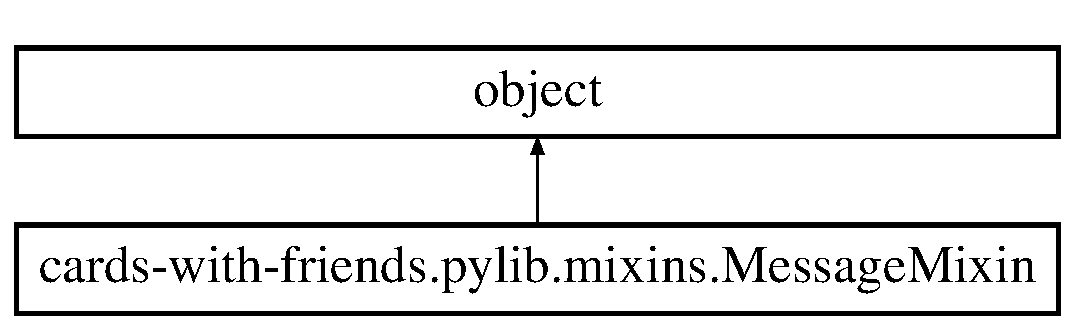
\includegraphics[height=2.000000cm]{classcards-with-friends_1_1pylib_1_1mixins_1_1_message_mixin}
\end{center}
\end{figure}
\subsection*{Public Member Functions}
\begin{DoxyCompactItemize}
\item 
\hypertarget{classcards-with-friends_1_1pylib_1_1mixins_1_1_message_mixin_ae55f0b8f15b7a839bec09f65a5e7b0d4}{def {\bfseries Receive\-Message}}\label{classcards-with-friends_1_1pylib_1_1mixins_1_1_message_mixin_ae55f0b8f15b7a839bec09f65a5e7b0d4}

\item 
\hypertarget{classcards-with-friends_1_1pylib_1_1mixins_1_1_message_mixin_ac62a3243d4de07bad9300b611b070127}{def {\bfseries Register\-Handler}}\label{classcards-with-friends_1_1pylib_1_1mixins_1_1_message_mixin_ac62a3243d4de07bad9300b611b070127}

\item 
\hypertarget{classcards-with-friends_1_1pylib_1_1mixins_1_1_message_mixin_aa0028b347cc219441ccad360781ff4e3}{def {\bfseries Send\-Message}}\label{classcards-with-friends_1_1pylib_1_1mixins_1_1_message_mixin_aa0028b347cc219441ccad360781ff4e3}

\item 
\hypertarget{classcards-with-friends_1_1pylib_1_1mixins_1_1_message_mixin_a12c18674923855655ccafdeb8da6ea46}{def {\bfseries Notify}}\label{classcards-with-friends_1_1pylib_1_1mixins_1_1_message_mixin_a12c18674923855655ccafdeb8da6ea46}

\item 
\hypertarget{classcards-with-friends_1_1pylib_1_1mixins_1_1_message_mixin_a0e4639ef11c326d3dc502a1d3d1a95ab}{def {\bfseries Request}}\label{classcards-with-friends_1_1pylib_1_1mixins_1_1_message_mixin_a0e4639ef11c326d3dc502a1d3d1a95ab}

\end{DoxyCompactItemize}


\subsection{Detailed Description}
\begin{DoxyVerb}Mixin for message-passing.\end{DoxyVerb}
 

The documentation for this class was generated from the following file\-:\begin{DoxyCompactItemize}
\item 
pylib/mixins.\-py\end{DoxyCompactItemize}

\hypertarget{classcards-with-friends_1_1player_1_1_player}{\section{cards-\/with-\/friends.player.\-Player Class Reference}
\label{classcards-with-friends_1_1player_1_1_player}\index{cards-\/with-\/friends.\-player.\-Player@{cards-\/with-\/friends.\-player.\-Player}}
}
Inheritance diagram for cards-\/with-\/friends.player.\-Player\-:\begin{figure}[H]
\begin{center}
\leavevmode
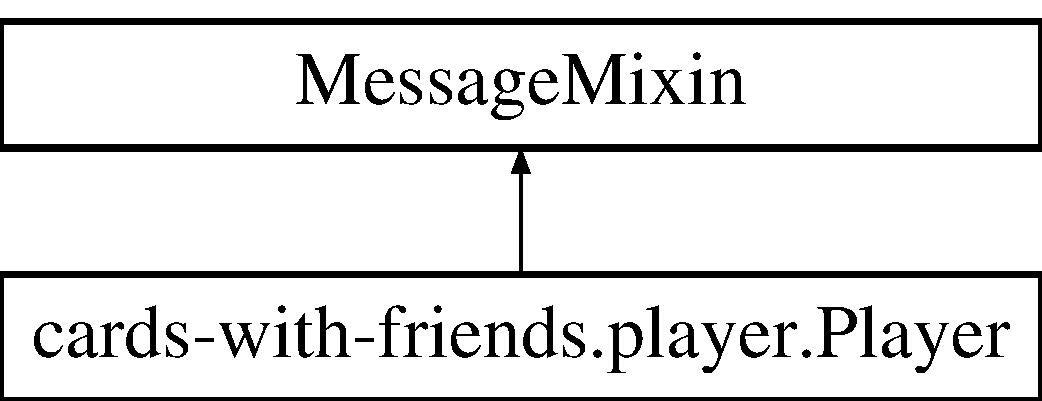
\includegraphics[height=2.000000cm]{classcards-with-friends_1_1player_1_1_player}
\end{center}
\end{figure}
\subsection*{Public Member Functions}
\begin{DoxyCompactItemize}
\item 
\hypertarget{classcards-with-friends_1_1player_1_1_player_a870653b97184fdf2b3d280335ad85a75}{def {\bfseries \-\_\-\-\_\-init\-\_\-\-\_\-}}\label{classcards-with-friends_1_1player_1_1_player_a870653b97184fdf2b3d280335ad85a75}

\item 
\hypertarget{classcards-with-friends_1_1player_1_1_player_ac7883932b882c801acba1fa20e82823f}{def {\bfseries \-\_\-\-\_\-repr\-\_\-\-\_\-}}\label{classcards-with-friends_1_1player_1_1_player_ac7883932b882c801acba1fa20e82823f}

\item 
def \hyperlink{classcards-with-friends_1_1player_1_1_player_aca27cc9aa97308913c5c3bab950337c9}{Add\-To\-Hand}
\item 
def \hyperlink{classcards-with-friends_1_1player_1_1_player_a76f414d3f246dbbe773a68b3f97406c3}{Add\-To\-Score}
\item 
def \hyperlink{classcards-with-friends_1_1player_1_1_player_a0942a5cfb0e6b67ba4fa865d1702136f}{Clear\-Hand}
\item 
def \hyperlink{classcards-with-friends_1_1player_1_1_player_aaee086f5336082c54312ddaea1b3fb32}{Clear\-Taken}
\item 
def \hyperlink{classcards-with-friends_1_1player_1_1_player_a2351ccc580354631fe7c54afdf1dae6e}{Get\-Bid}
\item 
def \hyperlink{classcards-with-friends_1_1player_1_1_player_a1aba66f48fc2a1f4b6f8e1720ee0ea7f}{Get\-Card}
\item 
def \hyperlink{classcards-with-friends_1_1player_1_1_player_a20ab5c7ed6517c5f325e1c34cfe23099}{Get\-Play}
\item 
def \hyperlink{classcards-with-friends_1_1player_1_1_player_ac43a65d18da6ad2a8b0b75bbce9b85f5}{Take}
\item 
\hypertarget{classcards-with-friends_1_1player_1_1_player_a88b7d8119bcf2e7e18c2a3539e5ea1bd}{def {\bfseries hand}}\label{classcards-with-friends_1_1player_1_1_player_a88b7d8119bcf2e7e18c2a3539e5ea1bd}

\item 
\hypertarget{classcards-with-friends_1_1player_1_1_player_aec146f8e7a9c6323dc39b3dd21b63e9a}{def {\bfseries id}}\label{classcards-with-friends_1_1player_1_1_player_aec146f8e7a9c6323dc39b3dd21b63e9a}

\item 
\hypertarget{classcards-with-friends_1_1player_1_1_player_a82f41ca09484367c16185d1df4b1bf32}{def {\bfseries money}}\label{classcards-with-friends_1_1player_1_1_player_a82f41ca09484367c16185d1df4b1bf32}

\item 
\hypertarget{classcards-with-friends_1_1player_1_1_player_a82f41ca09484367c16185d1df4b1bf32}{def {\bfseries money}}\label{classcards-with-friends_1_1player_1_1_player_a82f41ca09484367c16185d1df4b1bf32}

\item 
\hypertarget{classcards-with-friends_1_1player_1_1_player_a5f268545a8fcd20b97a629ce8f389cf7}{def {\bfseries name}}\label{classcards-with-friends_1_1player_1_1_player_a5f268545a8fcd20b97a629ce8f389cf7}

\item 
\hypertarget{classcards-with-friends_1_1player_1_1_player_a4c12918a7fe41459d67255b6bc07dfcb}{def {\bfseries score}}\label{classcards-with-friends_1_1player_1_1_player_a4c12918a7fe41459d67255b6bc07dfcb}

\item 
\hypertarget{classcards-with-friends_1_1player_1_1_player_a4c12918a7fe41459d67255b6bc07dfcb}{def {\bfseries score}}\label{classcards-with-friends_1_1player_1_1_player_a4c12918a7fe41459d67255b6bc07dfcb}

\item 
\hypertarget{classcards-with-friends_1_1player_1_1_player_a13de2ee2b5cc1e108ff6ee9862461281}{def {\bfseries taken}}\label{classcards-with-friends_1_1player_1_1_player_a13de2ee2b5cc1e108ff6ee9862461281}

\item 
\hypertarget{classcards-with-friends_1_1player_1_1_player_a13de2ee2b5cc1e108ff6ee9862461281}{def {\bfseries taken}}\label{classcards-with-friends_1_1player_1_1_player_a13de2ee2b5cc1e108ff6ee9862461281}

\end{DoxyCompactItemize}


\subsection{Detailed Description}
\begin{DoxyVerb}A player in a game.\end{DoxyVerb}
 

\subsection{Member Function Documentation}
\hypertarget{classcards-with-friends_1_1player_1_1_player_aca27cc9aa97308913c5c3bab950337c9}{\index{cards-\/with-\/friends\-::player\-::\-Player@{cards-\/with-\/friends\-::player\-::\-Player}!Add\-To\-Hand@{Add\-To\-Hand}}
\index{Add\-To\-Hand@{Add\-To\-Hand}!cards-with-friends::player::Player@{cards-\/with-\/friends\-::player\-::\-Player}}
\subsubsection[{Add\-To\-Hand}]{\setlength{\rightskip}{0pt plus 5cm}def cards-\/with-\/friends.\-player.\-Player.\-Add\-To\-Hand (
\begin{DoxyParamCaption}
\item[{}]{self, }
\item[{}]{cards}
\end{DoxyParamCaption}
)}}\label{classcards-with-friends_1_1player_1_1_player_aca27cc9aa97308913c5c3bab950337c9}
\begin{DoxyVerb}Add cards to the player's hand.\end{DoxyVerb}
 \hypertarget{classcards-with-friends_1_1player_1_1_player_a76f414d3f246dbbe773a68b3f97406c3}{\index{cards-\/with-\/friends\-::player\-::\-Player@{cards-\/with-\/friends\-::player\-::\-Player}!Add\-To\-Score@{Add\-To\-Score}}
\index{Add\-To\-Score@{Add\-To\-Score}!cards-with-friends::player::Player@{cards-\/with-\/friends\-::player\-::\-Player}}
\subsubsection[{Add\-To\-Score}]{\setlength{\rightskip}{0pt plus 5cm}def cards-\/with-\/friends.\-player.\-Player.\-Add\-To\-Score (
\begin{DoxyParamCaption}
\item[{}]{self, }
\item[{}]{score}
\end{DoxyParamCaption}
)}}\label{classcards-with-friends_1_1player_1_1_player_a76f414d3f246dbbe773a68b3f97406c3}
\begin{DoxyVerb}Add the specified amount to the player's current score.\end{DoxyVerb}
 \hypertarget{classcards-with-friends_1_1player_1_1_player_a0942a5cfb0e6b67ba4fa865d1702136f}{\index{cards-\/with-\/friends\-::player\-::\-Player@{cards-\/with-\/friends\-::player\-::\-Player}!Clear\-Hand@{Clear\-Hand}}
\index{Clear\-Hand@{Clear\-Hand}!cards-with-friends::player::Player@{cards-\/with-\/friends\-::player\-::\-Player}}
\subsubsection[{Clear\-Hand}]{\setlength{\rightskip}{0pt plus 5cm}def cards-\/with-\/friends.\-player.\-Player.\-Clear\-Hand (
\begin{DoxyParamCaption}
\item[{}]{self}
\end{DoxyParamCaption}
)}}\label{classcards-with-friends_1_1player_1_1_player_a0942a5cfb0e6b67ba4fa865d1702136f}
\begin{DoxyVerb}Clear the player's hand\end{DoxyVerb}
 \hypertarget{classcards-with-friends_1_1player_1_1_player_aaee086f5336082c54312ddaea1b3fb32}{\index{cards-\/with-\/friends\-::player\-::\-Player@{cards-\/with-\/friends\-::player\-::\-Player}!Clear\-Taken@{Clear\-Taken}}
\index{Clear\-Taken@{Clear\-Taken}!cards-with-friends::player::Player@{cards-\/with-\/friends\-::player\-::\-Player}}
\subsubsection[{Clear\-Taken}]{\setlength{\rightskip}{0pt plus 5cm}def cards-\/with-\/friends.\-player.\-Player.\-Clear\-Taken (
\begin{DoxyParamCaption}
\item[{}]{self}
\end{DoxyParamCaption}
)}}\label{classcards-with-friends_1_1player_1_1_player_aaee086f5336082c54312ddaea1b3fb32}
\begin{DoxyVerb}Clear the cards that the player has taken.\end{DoxyVerb}
 \hypertarget{classcards-with-friends_1_1player_1_1_player_a2351ccc580354631fe7c54afdf1dae6e}{\index{cards-\/with-\/friends\-::player\-::\-Player@{cards-\/with-\/friends\-::player\-::\-Player}!Get\-Bid@{Get\-Bid}}
\index{Get\-Bid@{Get\-Bid}!cards-with-friends::player::Player@{cards-\/with-\/friends\-::player\-::\-Player}}
\subsubsection[{Get\-Bid}]{\setlength{\rightskip}{0pt plus 5cm}def cards-\/with-\/friends.\-player.\-Player.\-Get\-Bid (
\begin{DoxyParamCaption}
\item[{}]{self, }
\item[{}]{message, }
\item[{}]{valid\-\_\-bids, }
\item[{}]{validator = {\ttfamily None}, }
\item[{}]{callback = {\ttfamily None}}
\end{DoxyParamCaption}
)}}\label{classcards-with-friends_1_1player_1_1_player_a2351ccc580354631fe7c54afdf1dae6e}
\begin{DoxyVerb}Get a bid from the player, given the message to tell them and the valid bids they can make.\end{DoxyVerb}
 \hypertarget{classcards-with-friends_1_1player_1_1_player_a1aba66f48fc2a1f4b6f8e1720ee0ea7f}{\index{cards-\/with-\/friends\-::player\-::\-Player@{cards-\/with-\/friends\-::player\-::\-Player}!Get\-Card@{Get\-Card}}
\index{Get\-Card@{Get\-Card}!cards-with-friends::player::Player@{cards-\/with-\/friends\-::player\-::\-Player}}
\subsubsection[{Get\-Card}]{\setlength{\rightskip}{0pt plus 5cm}def cards-\/with-\/friends.\-player.\-Player.\-Get\-Card (
\begin{DoxyParamCaption}
\item[{}]{self, }
\item[{}]{message, }
\item[{}]{valid\-\_\-cards, }
\item[{}]{num\-\_\-cards = {\ttfamily 1}, }
\item[{}]{validator = {\ttfamily None}, }
\item[{}]{callback = {\ttfamily None}}
\end{DoxyParamCaption}
)}}\label{classcards-with-friends_1_1player_1_1_player_a1aba66f48fc2a1f4b6f8e1720ee0ea7f}
\begin{DoxyVerb}Get cards from the player, given the message to tell them, the valid cards they can play, and the number of cards to play (default set to 1)\end{DoxyVerb}
 \hypertarget{classcards-with-friends_1_1player_1_1_player_a20ab5c7ed6517c5f325e1c34cfe23099}{\index{cards-\/with-\/friends\-::player\-::\-Player@{cards-\/with-\/friends\-::player\-::\-Player}!Get\-Play@{Get\-Play}}
\index{Get\-Play@{Get\-Play}!cards-with-friends::player::Player@{cards-\/with-\/friends\-::player\-::\-Player}}
\subsubsection[{Get\-Play}]{\setlength{\rightskip}{0pt plus 5cm}def cards-\/with-\/friends.\-player.\-Player.\-Get\-Play (
\begin{DoxyParamCaption}
\item[{}]{self, }
\item[{}]{message, }
\item[{}]{valid\-\_\-cards, }
\item[{}]{num\-\_\-cards = {\ttfamily 1}, }
\item[{}]{validator = {\ttfamily None}, }
\item[{}]{callback = {\ttfamily None}}
\end{DoxyParamCaption}
)}}\label{classcards-with-friends_1_1player_1_1_player_a20ab5c7ed6517c5f325e1c34cfe23099}
\begin{DoxyVerb}Get cards from the player, given the message to tell them, the valid cards they can play, and the number of cards to play (default set to 1)\end{DoxyVerb}
 \hypertarget{classcards-with-friends_1_1player_1_1_player_ac43a65d18da6ad2a8b0b75bbce9b85f5}{\index{cards-\/with-\/friends\-::player\-::\-Player@{cards-\/with-\/friends\-::player\-::\-Player}!Take@{Take}}
\index{Take@{Take}!cards-with-friends::player::Player@{cards-\/with-\/friends\-::player\-::\-Player}}
\subsubsection[{Take}]{\setlength{\rightskip}{0pt plus 5cm}def cards-\/with-\/friends.\-player.\-Player.\-Take (
\begin{DoxyParamCaption}
\item[{}]{self, }
\item[{}]{cards}
\end{DoxyParamCaption}
)}}\label{classcards-with-friends_1_1player_1_1_player_ac43a65d18da6ad2a8b0b75bbce9b85f5}
\begin{DoxyVerb}Add cards to the cards a player has taken.\end{DoxyVerb}
 

The documentation for this class was generated from the following file\-:\begin{DoxyCompactItemize}
\item 
player.\-py\end{DoxyCompactItemize}

\hypertarget{classcards-with-friends_1_1main_1_1_room}{\section{cards-\/with-\/friends.main.\-Room Class Reference}
\label{classcards-with-friends_1_1main_1_1_room}\index{cards-\/with-\/friends.\-main.\-Room@{cards-\/with-\/friends.\-main.\-Room}}
}
Inheritance diagram for cards-\/with-\/friends.main.\-Room\-:\begin{figure}[H]
\begin{center}
\leavevmode
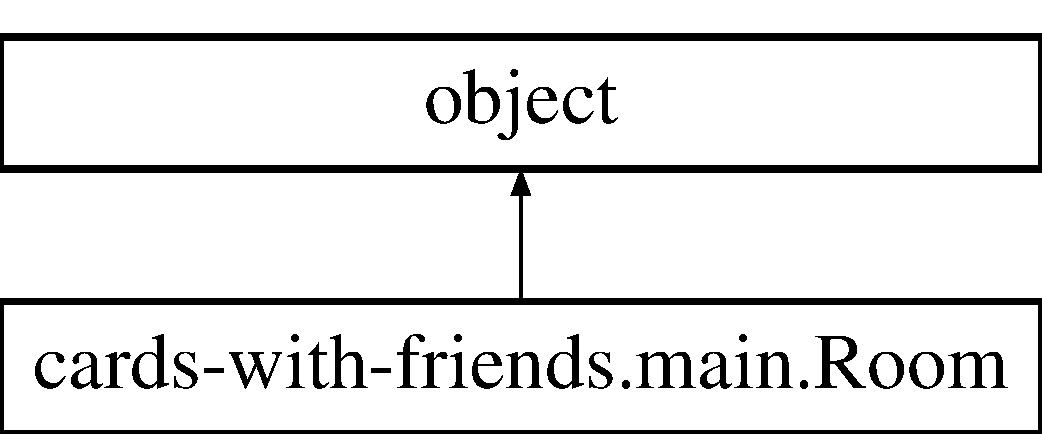
\includegraphics[height=2.000000cm]{classcards-with-friends_1_1main_1_1_room}
\end{center}
\end{figure}
\subsection*{Public Member Functions}
\begin{DoxyCompactItemize}
\item 
\hypertarget{classcards-with-friends_1_1main_1_1_room_ac299bcc847fb04e88cc2d617040d713d}{def {\bfseries \-\_\-\-\_\-init\-\_\-\-\_\-}}\label{classcards-with-friends_1_1main_1_1_room_ac299bcc847fb04e88cc2d617040d713d}

\item 
\hypertarget{classcards-with-friends_1_1main_1_1_room_a84ce168193a77212ae2bd63089d43867}{def {\bfseries full}}\label{classcards-with-friends_1_1main_1_1_room_a84ce168193a77212ae2bd63089d43867}

\item 
\hypertarget{classcards-with-friends_1_1main_1_1_room_a10f45f9f510a1903394259a659e0b374}{def {\bfseries num\-\_\-players}}\label{classcards-with-friends_1_1main_1_1_room_a10f45f9f510a1903394259a659e0b374}

\item 
\hypertarget{classcards-with-friends_1_1main_1_1_room_a03e7fd00e4ffe93adbbcb48fb35bd133}{def {\bfseries Add\-Player}}\label{classcards-with-friends_1_1main_1_1_room_a03e7fd00e4ffe93adbbcb48fb35bd133}

\item 
\hypertarget{classcards-with-friends_1_1main_1_1_room_ab325f2b38b1315a1e6ce367b55c1f77b}{def {\bfseries Remove\-Player}}\label{classcards-with-friends_1_1main_1_1_room_ab325f2b38b1315a1e6ce367b55c1f77b}

\item 
\hypertarget{classcards-with-friends_1_1main_1_1_room_a6df7c631f0179fe2c8202cebca309c74}{def {\bfseries Start\-Game}}\label{classcards-with-friends_1_1main_1_1_room_a6df7c631f0179fe2c8202cebca309c74}

\end{DoxyCompactItemize}
\subsection*{Public Attributes}
\begin{DoxyCompactItemize}
\item 
\hypertarget{classcards-with-friends_1_1main_1_1_room_aadc70adeea107495c7da140785db1b71}{{\bfseries id}}\label{classcards-with-friends_1_1main_1_1_room_aadc70adeea107495c7da140785db1b71}

\item 
\hypertarget{classcards-with-friends_1_1main_1_1_room_aab5bf3c72e42063b242b618c7dd807c9}{{\bfseries host}}\label{classcards-with-friends_1_1main_1_1_room_aab5bf3c72e42063b242b618c7dd807c9}

\item 
\hypertarget{classcards-with-friends_1_1main_1_1_room_a6c2c33b8796f1ea5d77d23e9441f343e}{{\bfseries game\-\_\-name}}\label{classcards-with-friends_1_1main_1_1_room_a6c2c33b8796f1ea5d77d23e9441f343e}

\item 
\hypertarget{classcards-with-friends_1_1main_1_1_room_a5fa1116257748fdde1d708ba7085013c}{{\bfseries players}}\label{classcards-with-friends_1_1main_1_1_room_a5fa1116257748fdde1d708ba7085013c}

\item 
\hypertarget{classcards-with-friends_1_1main_1_1_room_a5eb31d2acf2fcb13b398fe1393363d3d}{{\bfseries capacity}}\label{classcards-with-friends_1_1main_1_1_room_a5eb31d2acf2fcb13b398fe1393363d3d}

\item 
\hypertarget{classcards-with-friends_1_1main_1_1_room_a669025fad526c19ad37ef40cdb87e0de}{{\bfseries game}}\label{classcards-with-friends_1_1main_1_1_room_a669025fad526c19ad37ef40cdb87e0de}

\item 
\hypertarget{classcards-with-friends_1_1main_1_1_room_aa7b104fd42bbe4b7879fafcaa3c5cc67}{{\bfseries num\-\_\-players}}\label{classcards-with-friends_1_1main_1_1_room_aa7b104fd42bbe4b7879fafcaa3c5cc67}

\end{DoxyCompactItemize}


The documentation for this class was generated from the following file\-:\begin{DoxyCompactItemize}
\item 
main.\-py\end{DoxyCompactItemize}

\hypertarget{classcards-with-friends_1_1games_1_1spades_1_1_spades}{\section{cards-\/with-\/friends.games.\-spades.\-Spades Class Reference}
\label{classcards-with-friends_1_1games_1_1spades_1_1_spades}\index{cards-\/with-\/friends.\-games.\-spades.\-Spades@{cards-\/with-\/friends.\-games.\-spades.\-Spades}}
}
Inheritance diagram for cards-\/with-\/friends.games.\-spades.\-Spades\-:\begin{figure}[H]
\begin{center}
\leavevmode
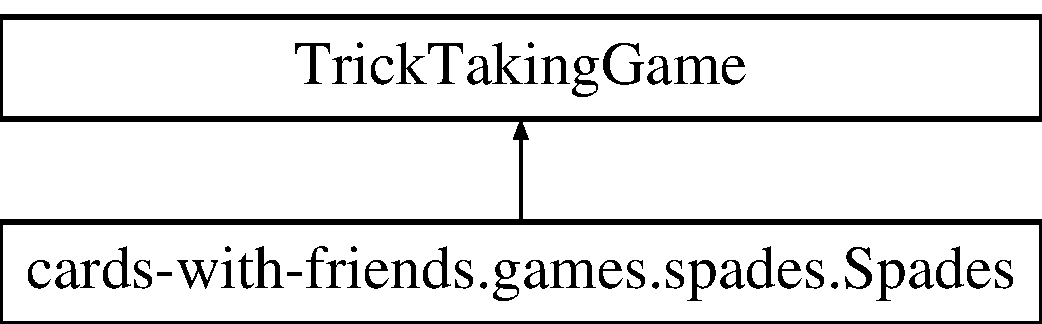
\includegraphics[height=2.000000cm]{classcards-with-friends_1_1games_1_1spades_1_1_spades}
\end{center}
\end{figure}
\subsection*{Public Member Functions}
\begin{DoxyCompactItemize}
\item 
\hypertarget{classcards-with-friends_1_1games_1_1spades_1_1_spades_a7588de7e14ab2dc26b08d371e800d94e}{def {\bfseries \-\_\-\-\_\-init\-\_\-\-\_\-}}\label{classcards-with-friends_1_1games_1_1spades_1_1_spades_a7588de7e14ab2dc26b08d371e800d94e}

\item 
def \hyperlink{classcards-with-friends_1_1games_1_1spades_1_1_spades_a4d88006569324913fb3410ab25195e5c}{Get\-Card\-Value}
\item 
def \hyperlink{classcards-with-friends_1_1games_1_1spades_1_1_spades_a06a9acc462f41d4eb61279c0ab6b09d7}{Play\-Game}
\item 
def \hyperlink{classcards-with-friends_1_1games_1_1spades_1_1_spades_a841395ddce5b12bee3d047dac25334ff}{Reset\-Game}
\end{DoxyCompactItemize}
\subsection*{Public Attributes}
\begin{DoxyCompactItemize}
\item 
\hypertarget{classcards-with-friends_1_1games_1_1spades_1_1_spades_a76ac0333f36b14b5fee950739b538676}{{\bfseries cards\-\_\-played}}\label{classcards-with-friends_1_1games_1_1spades_1_1_spades_a76ac0333f36b14b5fee950739b538676}

\item 
\hypertarget{classcards-with-friends_1_1games_1_1spades_1_1_spades_aca06f02693cd5d784a31305551b3d97f}{{\bfseries trick\-\_\-num}}\label{classcards-with-friends_1_1games_1_1spades_1_1_spades_aca06f02693cd5d784a31305551b3d97f}

\item 
\hypertarget{classcards-with-friends_1_1games_1_1spades_1_1_spades_a44d3c372f922d1c1fc2110f0531d1f57}{{\bfseries spades\-\_\-broken}}\label{classcards-with-friends_1_1games_1_1spades_1_1_spades_a44d3c372f922d1c1fc2110f0531d1f57}

\item 
\hypertarget{classcards-with-friends_1_1games_1_1spades_1_1_spades_a53aa57c30689ad752c41098d905debfc}{{\bfseries round\-\_\-num}}\label{classcards-with-friends_1_1games_1_1spades_1_1_spades_a53aa57c30689ad752c41098d905debfc}

\item 
\hypertarget{classcards-with-friends_1_1games_1_1spades_1_1_spades_a058680e817a07bd599fee2e9518b4464}{{\bfseries dealer}}\label{classcards-with-friends_1_1games_1_1spades_1_1_spades_a058680e817a07bd599fee2e9518b4464}

\end{DoxyCompactItemize}


\subsection{Detailed Description}
\begin{DoxyVerb}The Spades card game.\end{DoxyVerb}
 

\subsection{Member Function Documentation}
\hypertarget{classcards-with-friends_1_1games_1_1spades_1_1_spades_a4d88006569324913fb3410ab25195e5c}{\index{cards-\/with-\/friends\-::games\-::spades\-::\-Spades@{cards-\/with-\/friends\-::games\-::spades\-::\-Spades}!Get\-Card\-Value@{Get\-Card\-Value}}
\index{Get\-Card\-Value@{Get\-Card\-Value}!cards-with-friends::games::spades::Spades@{cards-\/with-\/friends\-::games\-::spades\-::\-Spades}}
\subsubsection[{Get\-Card\-Value}]{\setlength{\rightskip}{0pt plus 5cm}def cards-\/with-\/friends.\-games.\-spades.\-Spades.\-Get\-Card\-Value (
\begin{DoxyParamCaption}
\item[{}]{cls, }
\item[{}]{card}
\end{DoxyParamCaption}
)}}\label{classcards-with-friends_1_1games_1_1spades_1_1_spades_a4d88006569324913fb3410ab25195e5c}
\begin{DoxyVerb}Return the value of a card as prescribed by this game.\end{DoxyVerb}
 \hypertarget{classcards-with-friends_1_1games_1_1spades_1_1_spades_a06a9acc462f41d4eb61279c0ab6b09d7}{\index{cards-\/with-\/friends\-::games\-::spades\-::\-Spades@{cards-\/with-\/friends\-::games\-::spades\-::\-Spades}!Play\-Game@{Play\-Game}}
\index{Play\-Game@{Play\-Game}!cards-with-friends::games::spades::Spades@{cards-\/with-\/friends\-::games\-::spades\-::\-Spades}}
\subsubsection[{Play\-Game}]{\setlength{\rightskip}{0pt plus 5cm}def cards-\/with-\/friends.\-games.\-spades.\-Spades.\-Play\-Game (
\begin{DoxyParamCaption}
\item[{}]{self}
\end{DoxyParamCaption}
)}}\label{classcards-with-friends_1_1games_1_1spades_1_1_spades_a06a9acc462f41d4eb61279c0ab6b09d7}
\begin{DoxyVerb}Play the game.\end{DoxyVerb}
 \hypertarget{classcards-with-friends_1_1games_1_1spades_1_1_spades_a841395ddce5b12bee3d047dac25334ff}{\index{cards-\/with-\/friends\-::games\-::spades\-::\-Spades@{cards-\/with-\/friends\-::games\-::spades\-::\-Spades}!Reset\-Game@{Reset\-Game}}
\index{Reset\-Game@{Reset\-Game}!cards-with-friends::games::spades::Spades@{cards-\/with-\/friends\-::games\-::spades\-::\-Spades}}
\subsubsection[{Reset\-Game}]{\setlength{\rightskip}{0pt plus 5cm}def cards-\/with-\/friends.\-games.\-spades.\-Spades.\-Reset\-Game (
\begin{DoxyParamCaption}
\item[{}]{self}
\end{DoxyParamCaption}
)}}\label{classcards-with-friends_1_1games_1_1spades_1_1_spades_a841395ddce5b12bee3d047dac25334ff}
\begin{DoxyVerb}Reset the entire game state.\end{DoxyVerb}
 

The documentation for this class was generated from the following file\-:\begin{DoxyCompactItemize}
\item 
games/spades.\-py\end{DoxyCompactItemize}

\hypertarget{classcards-with-friends_1_1trick__taking__game_1_1_trick_taking_game}{\section{cards-\/with-\/friends.trick\-\_\-taking\-\_\-game.\-Trick\-Taking\-Game Class Reference}
\label{classcards-with-friends_1_1trick__taking__game_1_1_trick_taking_game}\index{cards-\/with-\/friends.\-trick\-\_\-taking\-\_\-game.\-Trick\-Taking\-Game@{cards-\/with-\/friends.\-trick\-\_\-taking\-\_\-game.\-Trick\-Taking\-Game}}
}
Inheritance diagram for cards-\/with-\/friends.trick\-\_\-taking\-\_\-game.\-Trick\-Taking\-Game\-:\begin{figure}[H]
\begin{center}
\leavevmode
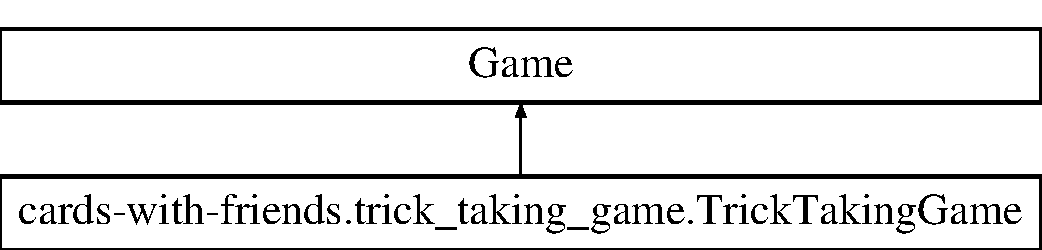
\includegraphics[height=2.000000cm]{classcards-with-friends_1_1trick__taking__game_1_1_trick_taking_game}
\end{center}
\end{figure}
\subsection*{Public Member Functions}
\begin{DoxyCompactItemize}
\item 
def \hyperlink{classcards-with-friends_1_1trick__taking__game_1_1_trick_taking_game_afd245781babd93951cf0dd612deb17d6}{\-\_\-\-\_\-init\-\_\-\-\_\-}
\item 
\hypertarget{classcards-with-friends_1_1trick__taking__game_1_1_trick_taking_game_a9389357f1f1838396c08c55363f17d68}{def {\bfseries Get\-Card\-Value}}\label{classcards-with-friends_1_1trick__taking__game_1_1_trick_taking_game_a9389357f1f1838396c08c55363f17d68}

\item 
def \hyperlink{classcards-with-friends_1_1trick__taking__game_1_1_trick_taking_game_a61a2f87ee4399c3d769f8feeff654521}{Sort\-Cards}
\item 
\hypertarget{classcards-with-friends_1_1trick__taking__game_1_1_trick_taking_game_ab6d7fb3479e1fe455aabf6d592c10581}{def {\bfseries Play\-Game}}\label{classcards-with-friends_1_1trick__taking__game_1_1_trick_taking_game_ab6d7fb3479e1fe455aabf6d592c10581}

\item 
\hypertarget{classcards-with-friends_1_1trick__taking__game_1_1_trick_taking_game_a93a0386100d04aa81a6d1bac32611c5b}{def {\bfseries Reset\-Game}}\label{classcards-with-friends_1_1trick__taking__game_1_1_trick_taking_game_a93a0386100d04aa81a6d1bac32611c5b}

\end{DoxyCompactItemize}


\subsection{Detailed Description}
\begin{DoxyVerb}A trick-taking game.\end{DoxyVerb}
 

\subsection{Constructor \& Destructor Documentation}
\hypertarget{classcards-with-friends_1_1trick__taking__game_1_1_trick_taking_game_afd245781babd93951cf0dd612deb17d6}{\index{cards-\/with-\/friends\-::trick\-\_\-taking\-\_\-game\-::\-Trick\-Taking\-Game@{cards-\/with-\/friends\-::trick\-\_\-taking\-\_\-game\-::\-Trick\-Taking\-Game}!\-\_\-\-\_\-init\-\_\-\-\_\-@{\-\_\-\-\_\-init\-\_\-\-\_\-}}
\index{\-\_\-\-\_\-init\-\_\-\-\_\-@{\-\_\-\-\_\-init\-\_\-\-\_\-}!cards-with-friends::trick_taking_game::TrickTakingGame@{cards-\/with-\/friends\-::trick\-\_\-taking\-\_\-game\-::\-Trick\-Taking\-Game}}
\subsubsection[{\-\_\-\-\_\-init\-\_\-\-\_\-}]{\setlength{\rightskip}{0pt plus 5cm}def cards-\/with-\/friends.\-trick\-\_\-taking\-\_\-game.\-Trick\-Taking\-Game.\-\_\-\-\_\-init\-\_\-\-\_\- (
\begin{DoxyParamCaption}
\item[{}]{self, }
\item[{}]{players, }
\item[{}]{deck}
\end{DoxyParamCaption}
)}}\label{classcards-with-friends_1_1trick__taking__game_1_1_trick_taking_game_afd245781babd93951cf0dd612deb17d6}
\begin{DoxyVerb}Constructor.

Args:
  players: A list of Player objects.
  deck: The name of the deck for this game.
\end{DoxyVerb}
 

\subsection{Member Function Documentation}
\hypertarget{classcards-with-friends_1_1trick__taking__game_1_1_trick_taking_game_a61a2f87ee4399c3d769f8feeff654521}{\index{cards-\/with-\/friends\-::trick\-\_\-taking\-\_\-game\-::\-Trick\-Taking\-Game@{cards-\/with-\/friends\-::trick\-\_\-taking\-\_\-game\-::\-Trick\-Taking\-Game}!Sort\-Cards@{Sort\-Cards}}
\index{Sort\-Cards@{Sort\-Cards}!cards-with-friends::trick_taking_game::TrickTakingGame@{cards-\/with-\/friends\-::trick\-\_\-taking\-\_\-game\-::\-Trick\-Taking\-Game}}
\subsubsection[{Sort\-Cards}]{\setlength{\rightskip}{0pt plus 5cm}def cards-\/with-\/friends.\-trick\-\_\-taking\-\_\-game.\-Trick\-Taking\-Game.\-Sort\-Cards (
\begin{DoxyParamCaption}
\item[{}]{cls, }
\item[{}]{cards, }
\item[{}]{reverse = {\ttfamily True}}
\end{DoxyParamCaption}
)}}\label{classcards-with-friends_1_1trick__taking__game_1_1_trick_taking_game_a61a2f87ee4399c3d769f8feeff654521}
\begin{DoxyVerb}Sort a list of cards by value. Returns an iterator.\end{DoxyVerb}
 

The documentation for this class was generated from the following file\-:\begin{DoxyCompactItemize}
\item 
trick\-\_\-taking\-\_\-game.\-py\end{DoxyCompactItemize}

%--- End generated contents ---

% Index
\newpage
\phantomsection
\addcontentsline{toc}{part}{Index}
\printindex

\end{document}
